% CAISc 2026 submission.
\documentclass{article}

\PassOptionsToPackage{numbers,compress,sort}{natbib}
\usepackage{caisc_2026}

\usepackage[utf8]{inputenc}
\usepackage[T1]{fontenc}
\usepackage{amsmath}
\usepackage{amssymb}
\usepackage{amsfonts}
\usepackage{graphicx}
\usepackage{booktabs}
\usepackage{nicefrac}
\usepackage{microtype}
\usepackage{xcolor}
\usepackage{hyperref}
\hypersetup{hidelinks}
\usepackage{url}

\title{Uncertainty-Aware Neural Surrogate for Parametric L-Bracket Stress Prediction}

\author{Anonymous Author(s)\\
Affiliation\\
Address\\
\texttt{email}\\
}

\begin{document}
\maketitle

\begin{abstract}
Neural surrogates for finite-element analysis (FEA) promise large
speedups for design-space exploration but return predictions without
telling the engineer when to trust them. The missing ingredient is a
calibrated reliability layer: a per-prediction interval that flags when
the surrogate should be trusted and when to defer back to the full
simulation. We build one for a parametric flat L-shaped corner bracket
(hereafter, the L-bracket) in 2D plane-stress linear elasticity,
combining a MeshGraphNets-style graph neural network (GNN) surrogate, a
5-member Deep Ensemble, and conformalized quantile regression (CQR). On
in-distribution (ID) test data the surrogate achieves $1.81\%$ per-node
mean absolute percentage error (MAPE), and the conformal layer meets
its coverage guarantee at every tested nominal level (80--95\%). On a
pre-registered out-of-distribution (OOD) set, accuracy degrades and
coverage drops below nominal, but the ensemble uncertainty signal more
than doubles --- enabling a defer-to-FEA rule that detects $58\%$ of
the hardest corner-OOD cases at a $5\%$ false-alarm rate. The
contribution is the evaluation methodology --- pre-registered OOD
testing, per-condition extrapolation audit, and a concrete
trust-or-defer decision rule --- not the individual components.
\end{abstract}

\section{Introduction}
\label{sec:intro}

FEA is the standard tool for stress prediction on structural parts, but
its cost per evaluation rules it out of tight-inner-loop design
workflows~\citep{maurizi2022gnn, pfaff2021meshgraphnets}. Neural
surrogates reduce per-evaluation cost from seconds or minutes to
milliseconds on a consumer GPU; GNNs are a particularly natural fit
because they operate on the native FEA mesh~\citep{pfaff2021meshgraphnets,
maurizi2022gnn, gladstone2024gnn}. A bare surrogate, however, returns a
prediction for every query in the design space, including queries for
which it has no training evidence. The missing ingredient is a
calibrated reliability layer: a per-prediction interval whose coverage
is documented and whose width is informative, so that the engineer can
trust the surrogate when the interval is tight and defer to FEA when it
is wide.

\textbf{Study part.} We study the L-bracket, a canonical thin
shelf-bracket with three stress
concentrators --- an inside fillet at the concave corner and two
through-holes (Figure~\ref{fig:bracket_photo}). The part is modelled in
2D plane-stress linear elasticity under a static shelf load, with three
free design parameters: the inside fillet radius $R$, the horizontal-flange
hole position $p$, and the flange width $W$.

\begin{figure}[t]
  \centering
  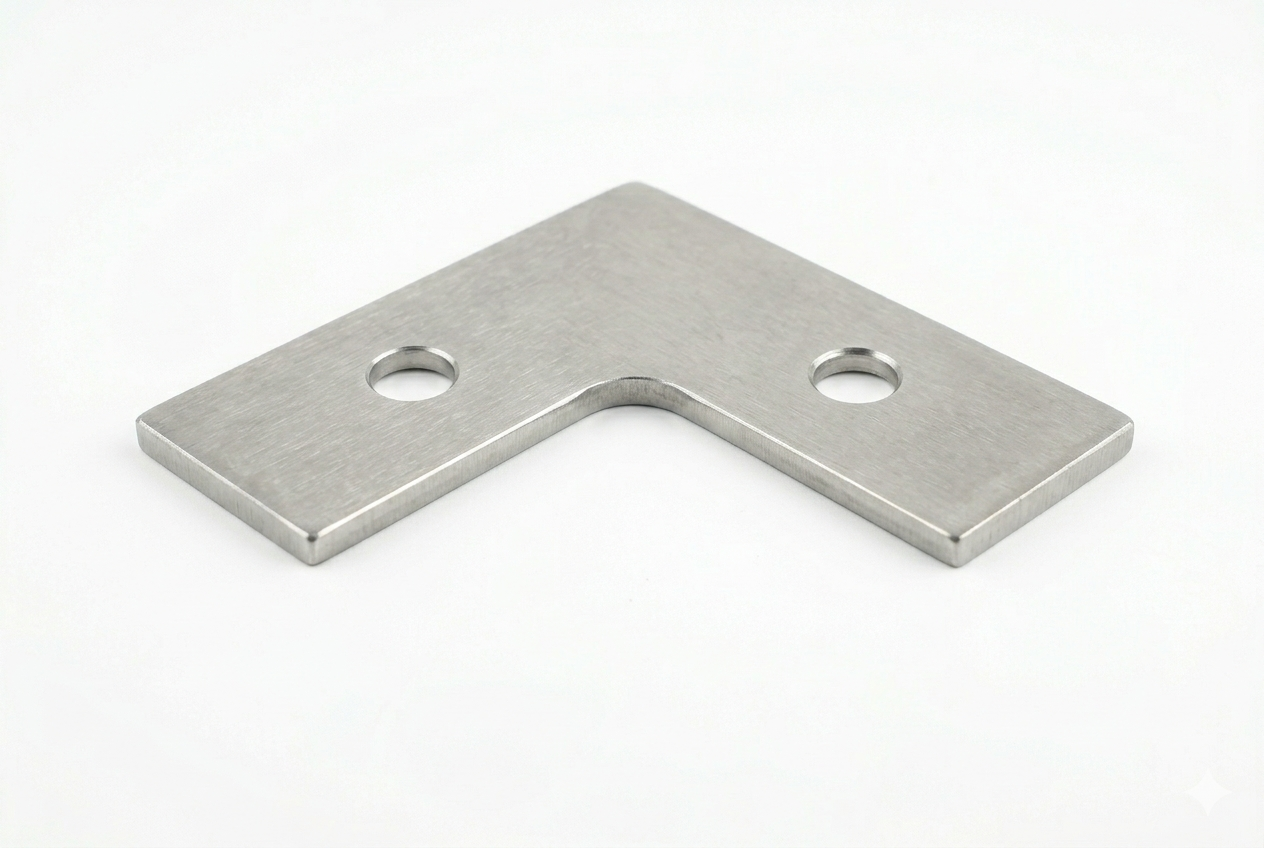
\includegraphics[width=0.5\linewidth]{figures/fig_bracket_photo.png}
  \caption{A flat L-shaped corner bracket in AISI 304 stainless steel,
    representative of the geometry studied in this work.}
  \label{fig:bracket_photo}
\end{figure}

\begin{figure}[t]
  \centering
  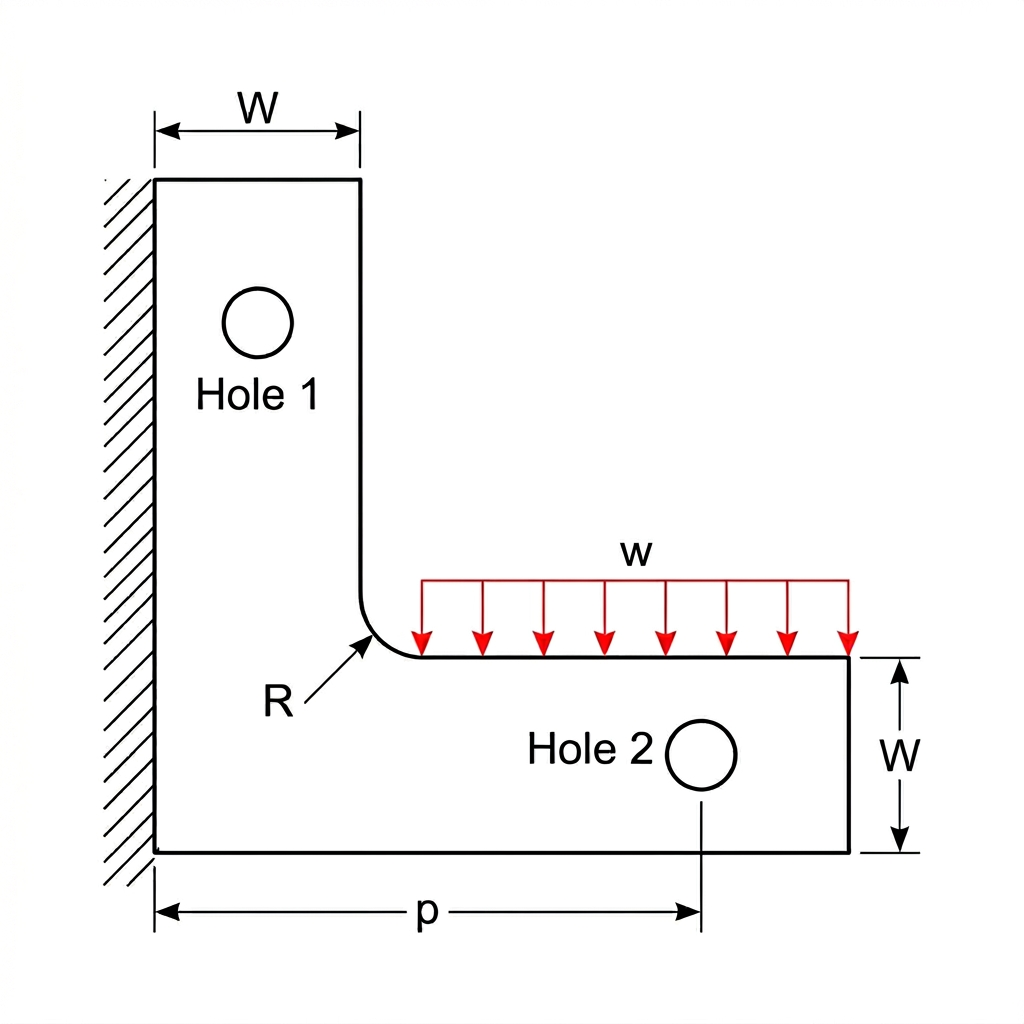
\includegraphics[width=0.7\linewidth]{figures/fig_geometry_schematic.png}
  \caption{Geometry and boundary conditions of the parametric
    L-bracket. $R$: inside fillet radius; $p$: Hole-2 position from the
    clamped face; $W$: flange width (symmetric). The back face of the
    vertical flange ($x = 0$) is fully clamped; a uniform shelf traction
    $w$ acts on the top face of the horizontal flange. (Lowercase $w$
    denotes the applied traction; uppercase $W$ denotes flange width.)}
  \label{fig:geometry_schematic}
\end{figure}

\textbf{Contribution.} The contribution of this paper is the reliability
layer, not the surrogate. We combine three well-established ingredients
--- a MeshGraphNets-style GNN~\citep{pfaff2021meshgraphnets,
maurizi2022gnn}, a Deep Ensemble for epistemic
uncertainty~\citep{lakshminarayanan2017ensembles}, and split-conformal
quantile regression~\citep{romano2019cqr, angelopoulos2023conformal,
gopakumar2024conformal} --- into a single deployment-calibrated
surrogate for parametric L-bracket stress prediction.
\citet{gopakumar2024conformal} demonstrate that cell-wise conformal
prediction provides marginal coverage guarantees for neural PDE
surrogates across several architectures. We build on their framework in
a stationary structural-mechanics setting where the mesh varies between
samples, and complement the coverage analysis with a pre-registered
out-of-distribution protocol, a per-condition extrapolation audit, and
a deployment-oriented deferral rule with quantified operating
characteristics. We verify the conformal coverage guarantee empirically
at four nominal levels on a held-out ID test set, show that accuracy
degrades and coverage drops on geometries outside the training box
while ensemble disagreement more than doubles, and present an
ensemble-size ablation that confirms the $M=5$ choice.

\section{Related Work}

Graph neural networks operate directly on unstructured FEA meshes and
predict solid-mechanics stress fields to within a few percent of the
reference~\citep{maurizi2022gnn, pfaff2021meshgraphnets,
gladstone2024gnn}. Uncertainty quantification for neural surrogates
splits into Bayesian approximations and post-hoc calibration
layers~\citep{psaros2023uq}; Deep
Ensembles~\citep{lakshminarayanan2017ensembles} are the dominant
practical choice for stress-field surrogates but the raw across-member
standard deviation carries no formal coverage guarantee. Conformal
prediction~\citep{angelopoulos2023conformal} converts any point or
interval predictor into a prediction interval with finite-sample,
distribution-free coverage under a single exchangeability assumption;
CQR~\citep{romano2019cqr} sharpens the split-conformal interval by
adapting its width to local heteroscedasticity.
\citet{gopakumar2024conformal} apply cell-wise conformal prediction to
neural PDE surrogates (multilayer perceptron, U-Net, Fourier neural operator, Vision Transformer, GNN) on time-dependent
spatio-temporal systems and study several nonconformity scores
including CQR. We adopt their cell-wise pooling recipe in a mesh-native
stationary structural-mechanics setting where the graph changes between
samples, and extend the coverage analysis with a pre-registered OOD
protocol, a per-condition extrapolation audit, and a deferral decision
rule with quantified operating characteristics. The present work
combines these ingredients: deep ensembles as the base predictor, CQR
as the calibration wrapper, and cell-wise pooling for node-level
marginal coverage on an FEA mesh.

\section{Methods}

\subsection{FEA problem setup}

The L-bracket is an equal-arm symmetric 2D plane-stress linear-elasticity
problem with three variable geometric parameters; fixed outer dimensions,
single AISI~304 stainless-steel material, and a static calibrated shelf
traction are summarized in Table~\ref{tab:setup}. The load magnitude
$w = 0.8555$~MPa is calibrated in a preliminary unit-load run on the
sample with the smallest fillet radius and narrowest flange width
($R = 3.0$~mm, $W = 14.0$~mm) --- the geometry producing the highest
stress concentration --- so that the peak von~Mises stress across the
sweep stays at $\sim 50\%$ of $\sigma_y$, keeping the full training set
in the elastic regime. Body forces, bolt-reaction contact at Hole~1, and the outside corner
fillet are omitted: all three are expected to contribute negligibly to
peak stress at this slenderness based on standard screening-level
sizing practice. Body forces are three orders of magnitude below the
applied traction; the outside corner lies on the compressive outer
bend and does not concentrate stress; bolt-reaction contact at Hole~1
is subsumed by the clamped-face idealization. Mesh convergence and an
analytical Euler--Bernoulli cross-check are reported in
Appendix~\ref{app:fea}.

\begin{table}[t]
  \centering
  \caption{Parametric L-bracket problem setup.}
  \label{tab:setup}
  \begin{tabular}{ll}
    \toprule
    Quantity & Value \\
    \midrule
    Arm lengths $A = B$ & $80$~mm \\
    Thickness $t$ (plane stress) & $8$~mm \\
    Hole diameter $D$ (both) & $8$~mm \\
    Fillet radius $R$ (swept) & $[3.0, 10.0]$~mm \\
    Hole-2 position $p$ (swept) & $[42.0, 72.0]$~mm \\
    Flange width $W$ (swept) & $[14.0, 24.0]$~mm \\
    Material & AISI 304 ($E = 193$~GPa, $\nu = 0.29$, $\sigma_y = 205$~MPa) \\
    Distributed shelf traction $w$ & $0.8555$~MPa (calibrated) \\
    Clamped boundary & back face of vertical flange ($x = 0$) \\
    FE scheme & FEniCSx, Lagrange order-2, $\sim 11{,}000$ degrees of freedom (DOF) \\
    Sampling & Latin Hypercube sampling (LHS)~\citep{mckay1979lhs}, 5000 in-distribution + 250 OOD \\
    Splits & 4000 train / 500 val / 500 test / 250 OOD \\
    \bottomrule
  \end{tabular}
\end{table}

\subsection{Surrogate architecture and training}

The surrogate is a MeshGraphNets-style
encoder--processor--decoder~\citep{pfaff2021meshgraphnets} adapted to
stationary stress prediction~\citep{maurizi2022gnn}. Each FEA sample is
one graph with 13 per-node features (2D coordinate, 6-way boundary-class
one-hot, the three design parameters $(R, p, W)$ broadcast as global
conditioning, and distances to the nearest fillet and hole-rim nodes)
and 4 per-edge features: the relative displacement vector
$(\Delta x, \Delta y)$, Euclidean length $\|\Delta\|$, and inverse
length $1/\|\Delta\|$.
The processor stacks $L=5$ residual message-passing blocks at hidden
width $H=128$ with sum aggregation; a node MLP decodes per-node von~Mises
stress in MPa. Training minimizes Huber loss~\citep{huber1964robust} ($\delta=1$~MPa) with Adam
(lr $5\times10^{-4}$ cosine-annealed to $10^{-5}$), batch size $8$, up to
60 epochs with patience 12 on validation loss. All training is performed
on a single NVIDIA RTX~4060 Laptop GPU (8~GB).

\subsection{Deep Ensembles and CQR}

Following Lakshminarayanan et
al.~\citep{lakshminarayanan2017ensembles}, we train a Deep Ensemble of
$M=5$ independently initialized members (differing only in random seed
and dataloader shuffle); at inference the ensemble mean
$\bar{\sigma}(\mathbf{x}_i)$ is the point estimate and the across-member
standard deviation $s(\mathbf{x}_i)$ is the epistemic-uncertainty scalar.

We convert $(\bar{\sigma}, s)$ into base quantile predictors via a
Gaussian ansatz, $\hat{q}_{\text{lo/hi}} = \bar{\sigma} \mp
z_{1-\alpha/2}\,s$. For a linear-elastic problem with smooth parameter
dependence, the ensemble-member predictions at each node are
approximately normally distributed around the mean, so the Gaussian
quantile rule is a reasonable starting point; the subsequent CQR
calibration step corrects any residual miscalibration introduced by
this assumption. We then apply split-conformal calibration (Algorithm~1
of Romano et al.~\citep{romano2019cqr}): on the 500-sample validation
calibration set we compute the CQR nonconformity score $E_{ij} =
\max(\hat{q}_{\text{lo}} - \sigma^\star,\, \sigma^\star -
\hat{q}_{\text{hi}})$, pool scores across all nodes of all calibration
samples into a single set (cell-wise
pooling~\citep{gopakumar2024conformal}: each node prediction is
treated as an independent exchangeable unit), and take
$\hat{Q}(\alpha) = \operatorname{Quantile}_{\lceil (n+1)(1-\alpha)
\rceil/n}(\{E_{ij}\})$. The final interval is $[\hat{q}_{\text{lo}} -
\hat{Q},\, \hat{q}_{\text{hi}} + \hat{Q}]$, carrying the Theorem~1
finite-sample coverage guarantee under exchangeability. Our 500-sample
validation set was previously used for a three-candidate hyperparameter
selection on point accuracy, inducing a bounded optimistic bias on
coverage: we acknowledge this reuse; the three-candidate selection
limits the degree of adaptation.

\subsection{Pre-registered OOD protocol}
\label{ssec:ood-protocol}

To make the extrapolation evaluation falsifiable, the OOD protocol was
fixed in writing before any model was trained.\footnote{The protocol
was committed to the project version-control repository before any
surrogate training began; the git commit timestamp serves as the
pre-registration artifact. The protocol document and commit hash will
be included in the public code release.} Each parameter is extended
$\pm 20\%$ of its training span beyond the training bound (clipped at
binding geometric constraints). 250 samples are allocated as 25 per
single-parameter direction (6 directions, 150 total) plus 100
corner-OOD samples where $\geq 2$ parameters are simultaneously outside
the training box. All Phase-1 and Phase-2 metrics are re-computed on this
set verbatim; no post-hoc exclusion is permitted.

\subsection{Deferral decision rule}
\label{ssec:deferral}

For deployment we threshold the per-sample mean ensemble standard
deviation $\bar{s}(\mathbf{x})$: use the surrogate when
$\bar{s} < T^\star$, defer to FEA otherwise. The threshold is the
$95^{\text{th}}$ percentile of $\bar{s}$ on the ID test set, giving $5\%$
ID false-alarm by construction.

\section{Results}
\label{sec:results}

\subsection{Surrogate accuracy and ensemble calibration}

On the 500-sample ID test set, the ensemble-mean prediction attains
$\mathbf{1.81\%}$ per-node and $\mathbf{0.42\%}$ peak-stress MAPE, with
median absolute error $0.032$~MPa and $99^{\text{th}}$ percentile
$0.32$~MPa (full per-seed breakdown in
Appendix~\ref{app:perseed}). The gap between the two MAPE figures is
expected: per-node MAPE pools thousands of low-stress nodes where small
absolute errors inflate percentage errors, whereas peak stress always
occurs at the fillet in every training sample, so ensemble averaging
at that consistently-located peak node reduces variance very
efficiently. An ensemble-size ablation
(Appendix~\ref{app:ensemble-ablation}) confirms that $M=5$ outperforms
smaller ensembles on both accuracy and calibration quality. The central Phase-1 claim --- that ensemble
disagreement tracks actual error --- is confirmed at both granularities:
node-level Pearson $0.494$ (Spearman $0.524$) and sample-level Pearson
$\mathbf{0.944}$ between ensemble std and absolute residual
(Figure~\ref{fig:phase1-calib}). Sample-level correlation is the number
the Phase-2 CQR layer inherits.

\begin{figure}[t]
  \centering
  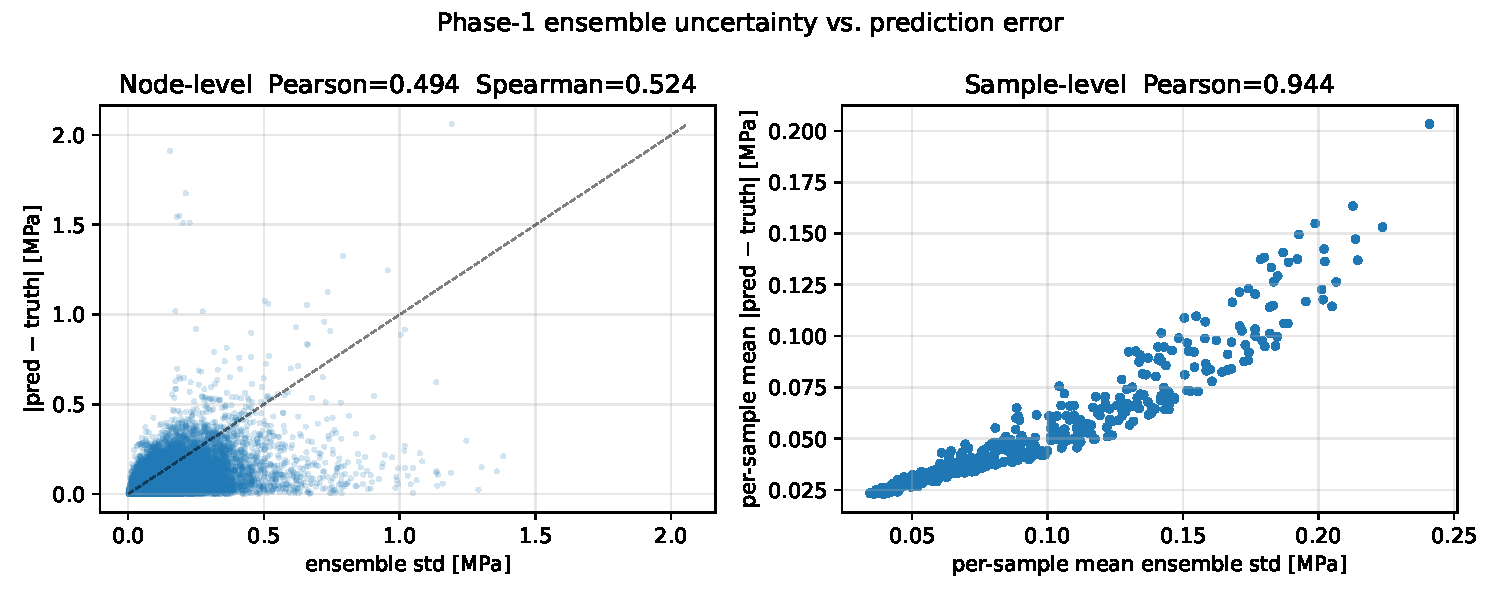
\includegraphics[width=\linewidth]{figures/fig_phase1_calibration.pdf}
  \caption{Ensemble uncertainty (x) vs.\ absolute error (y). \emph{Left:}
    node-level over all test-set nodes. \emph{Right:} per-sample scatter;
    each point is the mean uncertainty and mean error over one test
    sample. The strong sample-level trend is the empirical foundation
    for the Phase-2 CQR interval.}
  \label{fig:phase1-calib}
\end{figure}

\subsection{CQR coverage on the held-out test set}
\label{ssec:results-cqr}

Table~\ref{tab:coverage} reports empirical coverage at three
representative nominal levels for both the raw Gaussian ensemble
interval and the CQR-calibrated interval, evaluated once on the
held-out test set; the full four-level sweep
(80/85/90/95) is in Appendix~\ref{app:cqr}.

\begin{table}[t]
  \centering
  \caption{Empirical coverage and mean interval width on the ID test set
    (pooled across $\sim 1.56\times 10^{6}$ nodes), for the Gaussian
    ensemble interval $\bar{\sigma} \pm z_{1-\alpha/2}s$ and the
    CQR-calibrated interval; $\hat{Q}$ is the conformal correction
    learned on the 500-sample validation set. Full four-level sweep and
    conditional coverage in Appendix~\ref{app:cqr}.}
  \label{tab:coverage}
  \begin{tabular}{cccccc}
    \toprule
    Nominal [\%] &
    \multicolumn{2}{c}{Uncalibrated (Gaussian)} &
    \multicolumn{2}{c}{CQR-calibrated} &
    $\hat{Q}$ [MPa] \\
    \cmidrule(lr){2-3}\cmidrule(lr){4-5}
    & Coverage & Width [MPa] & Coverage & Width [MPa] & \\
    \midrule
    80 & 86.41 & 0.25 & 82.72 & 0.24 & $-0.005$ \\
    90 & 92.32 & 0.32 & 91.28 & 0.31 & $-0.003$ \\
    95 & 95.19 & 0.38 & 95.53 & 0.38 & $\phantom{-}0.001$ \\
    \bottomrule
  \end{tabular}
\end{table}

At every tested level the CQR interval attains at or above its nominal
coverage, consistent with Theorem~1 of \citet{romano2019cqr}
(Figure~\ref{fig:phase2-coverage}). The
conformal correction $\hat{Q}$ is sub-MPa and signed: CQR tightens the
over-wide small-$\alpha$ interval and widens the under-wide $95\%$
interval. Conditional coverage sliced by parameter quartile stays within
$\pm 3$~pp of nominal across all twelve quartiles
(Appendix~\ref{app:cqr}). Per-sample interval width correlates with
per-sample absolute error at Pearson $0.944$ --- the
deployment-relevant property (this correlation is inherited from the
ensemble-std signal already plotted in
Figure~\ref{fig:phase1-calib}, since CQR adds a constant correction
$\hat{Q}$ that does not affect the ranking of samples by width).
Against a vanilla split-conformal baseline calibrated on the same
validation pool (symmetric constant-width interval $\bar{\sigma}\pm
Q_{\text{vanilla}}$, using $|\bar{\sigma}-\sigma^\star|$ as the
nonconformity score), CQR delivers coverage at nominal while vanilla
under-covers ($81.1\%$ vs.\ $91.3\%$ at $\alpha=0.10$) despite using a
narrower $2Q_{\text{vanilla}} = 0.167$~MPa interval --- the adaptive
CQR width absorbs the within-sample node correlation that the
constant-width vanilla interval cannot. Full comparison in
Appendix~\ref{app:vanilla}. Having established that the CQR layer
delivers calibrated intervals on in-distribution data, we now evaluate
the full pipeline on geometries outside the training range.

\begin{figure}[t]
  \centering
  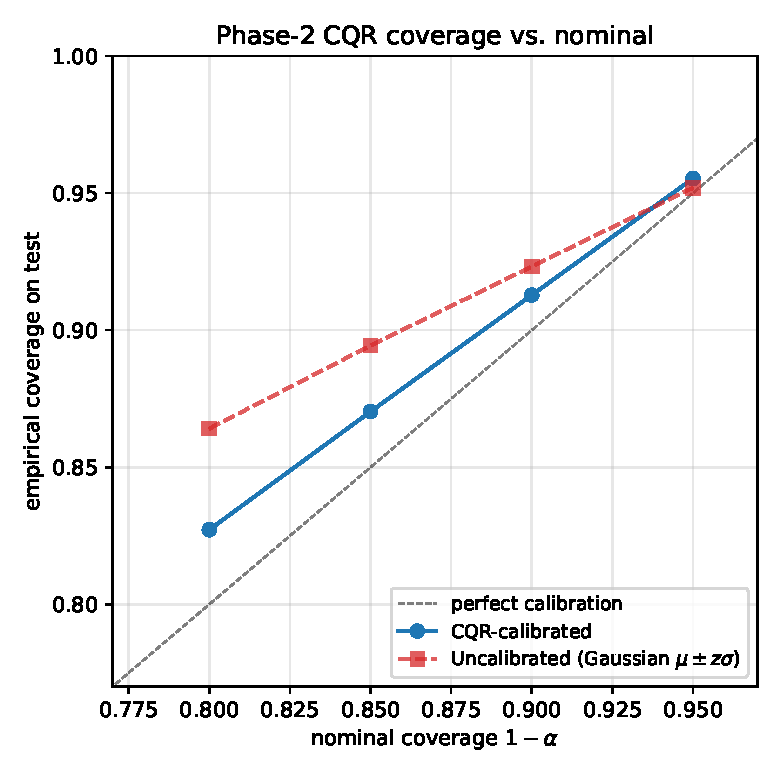
\includegraphics[width=0.55\linewidth]{figures/fig_phase2_coverage.pdf}
  \caption{Empirical vs.\ nominal coverage. Diagonal is perfect
    calibration. CQR tracks the diagonal from above at every level, as
    required by the Theorem~1 guarantee.}
  \label{fig:phase2-coverage}
\end{figure}

\subsection{Out-of-distribution evaluation}

The CQR-calibrated ensemble, frozen after Phase~2, is evaluated verbatim
on the 250 pre-registered OOD samples
(Table~\ref{tab:phase3-id-vs-ood}). Three findings. (i)~Accuracy
degrades: per-node MAPE $1.7\times$, peak-stress MAPE $17\times$ (both
ratios are full-OOD relative to ID); the disproportionate peak
degradation reflects OOD geometries whose stress
concentrators are sharper than any training sample. (ii)~CQR coverage
drops below nominal ($83.7\%$ vs.\ $90\%$), the expected finite-sample
realization of Theorem~1 losing its exchangeability premise.
(iii)~\textbf{The reliability layer scales up correctly}: mean CQR width
roughly doubles and mean ensemble std more than doubles. The reliability
layer produces a loud, measurable signal of degradation rather than
failing silently.

\begin{table}[t]
  \centering
  \caption{ID test vs.\ pre-registered OOD at nominal $90\%$ coverage.
    ID: $N=500$, $1.56\times 10^{6}$ nodes; OOD: $N=250$, $7.15\times
    10^{5}$ nodes. Per-condition OOD breakdown in
    Appendix~\ref{app:ood}.}
  \label{tab:phase3-id-vs-ood}
  \begin{tabular}{lccc}
    \toprule
    Metric & ID test & OOD & Change \\
    \midrule
    Per-node MAPE [\%] & 1.81 & 3.10 & 1.7$\times$ \\
    Peak-stress MAPE [\%] & 0.42 & 7.26 & 17$\times$ \\
    CQR coverage at 90\% [\%] & 91.28 & 83.70 & $-7.58$~pp \\
    CQR mean interval width [MPa] & 0.311 & 0.654 & 2.1$\times$ \\
    Mean ensemble std [MPa] & 0.096 & 0.208 & 2.2$\times$ \\
    \bottomrule
  \end{tabular}
\end{table}

The per-condition breakdown (Appendix~\ref{app:ood},
Table~\ref{tab:phase3-conditional}) is informative: $R$-low and
$R$-high extrapolations are handled essentially as well as ID
($\leq 1.3\%$ per-node MAPE, coverage within 2~pp, ensemble std at the ID
baseline), while both $p$ directions, $W$-low, and corner-OOD samples
drive the aggregate degradation. Corner OOD shows $4.56\%$ per-node
MAPE ($2.5\times$ ID), coverage $81.5\%$, and $3.5\times$ ensemble std.

\subsection{Example predictions}

Figure~\ref{fig:phase1-examples} shows best, median, and worst test
samples ranked by per-sample mean absolute error. The fillet --- the
dominant stress concentrator --- is recovered faithfully across the
three quantiles; residual error concentrates on the fillet arc and hole
rims, consistent with the literature-reported tail-compression pattern
of GNN mesh surrogates~\citep{maurizi2022gnn, gladstone2024gnn}. Critically,
the per-node ensemble std (right column) tracks the error map: the GNN
knows where it is less reliable.

\begin{figure}[t]
  \centering
  \makebox[\linewidth][c]{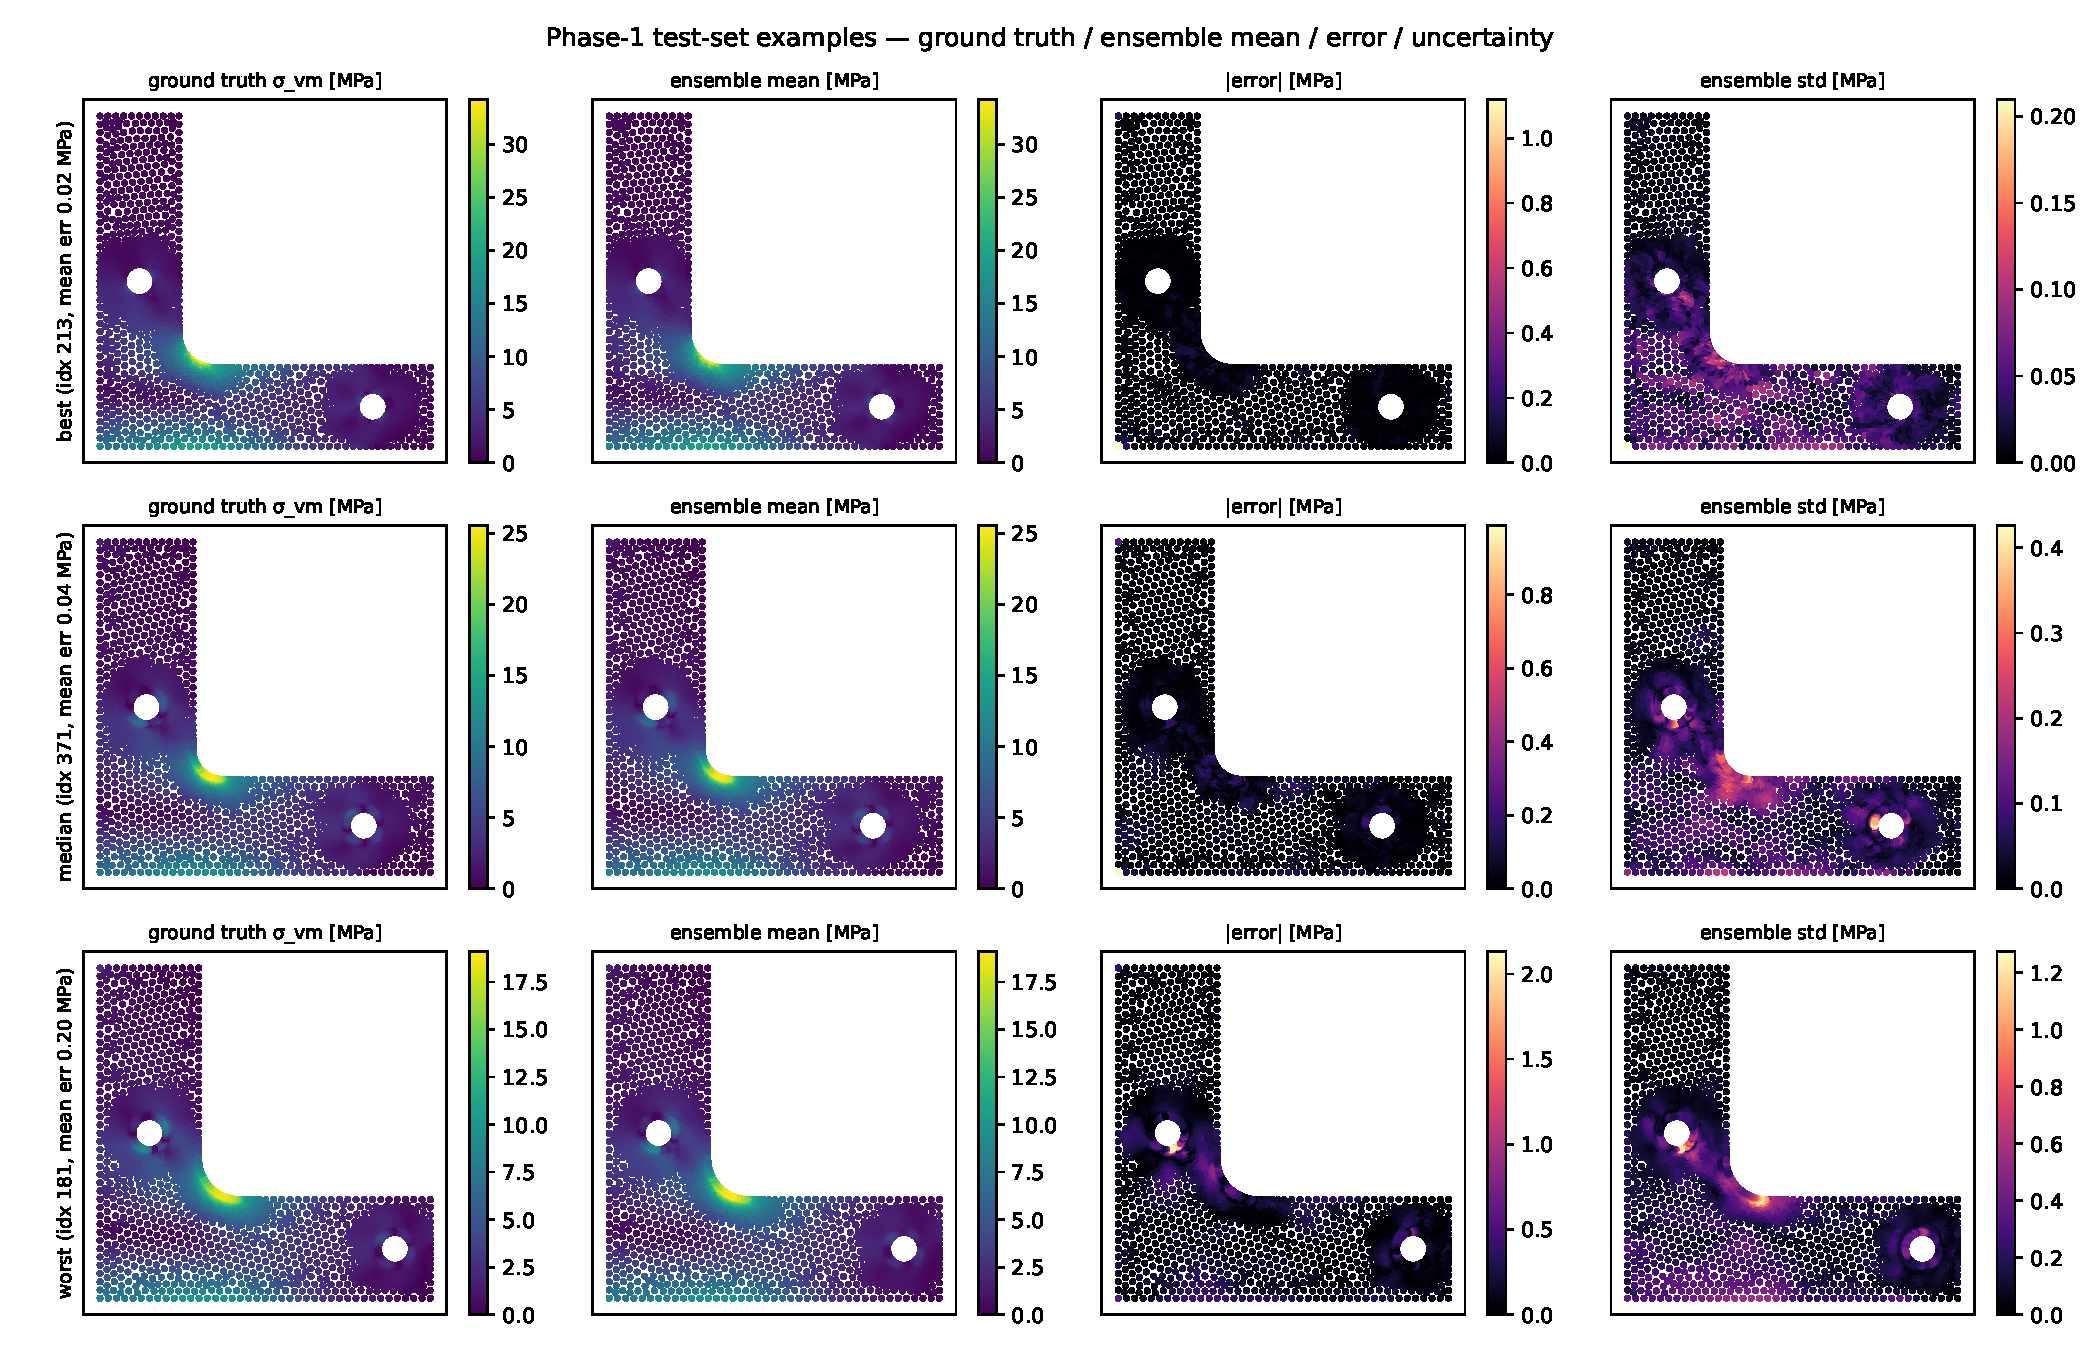
\includegraphics[width=1.15\linewidth]{figures/fig_phase1_example_predictions.pdf}}
  \caption{Test-set examples (best, median, worst by per-sample mean
    error). Columns: ground-truth von~Mises stress; ensemble-mean
    prediction; absolute error; ensemble standard deviation. The
    uncertainty map tracks the error map.}
  \label{fig:phase1-examples}
\end{figure}

\subsection{Defer-to-FEA decision rule}

At $T^\star = 0.182$~MPa (ID $95^{\text{th}}$ percentile of $\bar{s}$),
the rule flags $5\%$ of ID samples (false alarm, by construction) and
detects $34\%$ of the full OOD set and $\mathbf{58\%}$ of the
hardest corner-OOD condition. Per-condition detection is $0\%$ on the
$R$-direction perturbations (where the surrogate legitimately
extrapolates cleanly) and $4$--$44\%$ on the remaining single-parameter
conditions. The area under the receiver operating characteristic curve (AUROC) of
$\bar{s}$ as an OOD detector is $0.673$; some OOD conditions are in
practice easier for the surrogate than the hardest ID quartile
(Appendix~\ref{app:deferral}, Figure~\ref{fig:phase3-deferral-roc}).

\section{Discussion}

\paragraph{What CQR adds.} Ensemble disagreement alone is a scalar
without a probabilistic interpretation: in principle, two ensembles
with identical Pearson correlation to the truth can produce
differently calibrated intervals. CQR converts that signal into a prediction interval with a
distribution-free finite-sample coverage guarantee. For the L-bracket
the raw Gaussian interval is already close to calibrated and the
conformal correction remains sub-MPa --- this is a friendly case where
CQR's contribution is modest in magnitude but categorical in
interpretation.

\paragraph{Which extrapolation axes are safe.} The per-condition
breakdown (Appendix~\ref{app:ood}) carries a concrete engineering
message: on this geometry the surrogate extrapolates cleanly on
$R$ in both directions but not on $p$ or $W$, and not at all on joint
extrapolation. Any similar surrogate rollout should publish this
per-axis extrapolation audit alongside the headline accuracy number.

\paragraph{Limitations.} (i)~Coverage is marginal, not conditional;
covariate-shift conformal extensions~\citep{angelopoulos2023conformal}
would formalize the OOD case. (ii)~The calibration set doubles as the
Phase-1 hyperparameter-selection set; adaptation is bounded but not
zero. (iii)~Cell-wise pooling treats mesh nodes within a graph as
exchangeable, which they strictly are not. (iv)~No aleatoric head: the
FEA target is noise-free, so the reliability layer captures only
epistemic uncertainty. (v)~The physical model is idealized (2D plane
stress, single material, linear elasticity, no self-weight); relaxing
any of these requires re-calibration. (vi)~OOD is $\pm 20\%$
parametric extrapolation; structural extrapolation (new topology) is
out of scope.

\paragraph{Scalability.} The conformal calibration and ensemble
components add constant multiplicative overhead to the base surrogate
and impose no architectural constraints. In our experiments, CQR
calibration over 1.5 million pooled nonconformity scores completed in
seconds, with FEA data generation remaining the computational
bottleneck rather than the UQ layer. The framework thus transfers
directly to larger meshes and additional ensemble members; empirical
validation on higher-dimensional parametric families remains future
work.

\paragraph{Future work.} Asymmetric-arm brackets and higher-dimensional
parametric families, multiple load cases, nonlinear material response,
and 3D extension. A continuous covariate-shift-aware
recalibration~\citep{angelopoulos2023conformal} would replace the
binary deferral rule with a smoothly widened interval as the input
drifts from the training distribution.

\section{Conclusion}

We built a deployment-calibrated neural surrogate for parametric
L-bracket stress prediction by stacking a MeshGraphNets-style GNN, a
5-member Deep Ensemble, and a split-conformalized quantile-regression
layer on a common FEA training set. The surrogate attains $1.81\%$
per-node and $0.42\%$ peak-stress MAPE; the conformal layer delivers
the Romano~2019 Theorem~1 guarantee at every tested nominal level; the
interval width is informative at Pearson $0.944$ per sample. On a
pre-registered OOD set the guarantee expires as predicted but the
reliability layer's own signal more than doubles, yielding a
defer-to-FEA rule that detects $58\%$ of corner-OOD samples at $5\%$
ID false-alarm. The contribution is the combination and the honest
evaluation under a pre-registered protocol: a reliability retrofit that
is already deployable with today's standard UQ machinery.

\bibliographystyle{plainnat}
\bibliography{bibliography}

\newpage

\section*{Conference For AI Scientists 2026 - AI Involvement Checklist}
\label{checklist_ai_involvement}

\subsection*{Research Stage Assessment}

For items 1-4, give a score from the scale below that defines the role of AI in each part of the scientific process. The scores are as follows:

\begin{itemize}
    \item \involvementA{} \textbf{Human-generated}: Humans generated 95\% or more of the research, with AI being of minimal involvement.
    \item \involvementB{} \textbf{Mostly human, assisted by AI}: The research was a collaboration between humans and AI models, but humans produced the majority (>50\%) of the research.
    \item \involvementC{} \textbf{Mostly AI, assisted by human}: The research task was a collaboration between humans and AI models, but AI produced the majority (>50\%) of the research.
    \item \involvementD{} \textbf{AI-generated}: AI performed over 95\% of the research. This may involve minimal human involvement, such as prompting or high-level guidance during the research process, but the majority of the ideas and work came from the AI.
\end{itemize}

For each research stage where AI was involved, i.e. where you selected \involvementB{}, \involvementC{}, or \involvementD{}, please also indicate the approximate level of iteration effort required using the provided iteration macros. Count substantive attempts, prompts, runs, agent trajectories, or course corrections; do not count minor wording edits.

\begin{itemize}
    \item \iterationLow{}: approximately 1-10 substantive attempts.
    \item \iterationMedium{}: approximately 10-100 substantive attempts, with some failed attempts or course corrections.
    \item \iterationHigh{}: approximately 100+ substantive attempts, with substantial exploration, failures, or trial-and-error.
    \item \iterationNA{}: not applicable because AI involvement was \involvementA{}.
    \item \iterationUnclear{}: the authors cannot reasonably estimate.
\end{itemize}

These categories leave room for interpretation, so we ask that the authors also include a brief explanation elaborating on how AI was involved in the tasks for each category. Please keep your explanation to less than 150 words.

\begin{enumerate}

    \item \textbf{Hypothesis development}: Hypothesis development includes the process by which you came to explore this research topic and research question. This can involve the background research performed by either researchers or by AI. This can also involve whether the idea was proposed by researchers or by AI.

    Answer: \involvementB{}

    Iteration Effort: \iterationMedium{}

    Explanation: The research direction (uncertainty quantification for a structural neural surrogate) was identified through extended human--AI discussion spanning multiple sessions. The human author brought the domain expertise (mechanical engineering, bracket sizing practice) and the strategic framing (deployment reliability rather than surrogate accuracy as the contribution). The AI partner contributed literature grounding, landscape analysis of UQ methods, and helped narrow from a broad ``physical AI'' theme to the specific L-bracket UQ formulation. Two earlier project directions were abandoned after substantive investigation before the present scope was settled; the final choice of a GNN + Deep Ensemble + CQR stack emerged from iterated human--AI deliberation rather than a single prompt.

    \item \textbf{Experimental design and implementation}: This category includes design of experiments that are used to test the hypotheses, coding and implementation of computational methods, and the execution of these experiments.

    Answer: \involvementC{}

    Iteration Effort: \iterationHigh{}

    Explanation: An AI coding agent implemented the full pipeline: the FEniCSx FEA driver, the Latin-Hypercube parametric sweep, the MeshGraphNets-style GNN, the Deep Ensemble training loop, the split-conformal calibration, the pre-registered OOD sweep, and the deferral decision rule. The human author made the architectural and methodological decisions (GNN vs.\ CNN, 5-member ensemble size, CQR over MC Dropout, parameter ranges, material selection, single load case, 2D plane-stress reduction) and directed the agent to execute them. High iteration count: four failed attempts at a remote-compute sweep (install hang, captured-stdout silence, browser-lag firehose, recursive spawn deadlock) preceded the pivot to local WSL2 execution; the final local pipeline was reached after dozens of debugging cycles.

    \item \textbf{Analysis of data and interpretation of results}: This category encompasses any process to organize and process data for the experiments in the paper. It also includes interpretations of the results of the study.

    Answer: \involvementB{}

    Iteration Effort: \iterationMedium{}

    Explanation: The AI agent generated all analysis scripts, figures, tables, and summary statistics (accuracy metrics, coverage sweeps, conditional coverage tables, OOD breakdown, deferral ROC). The human author drove interpretation: what the sample-level Pearson $0.944$ implies for deployment trust, how the peak-stress MAPE blow-up on OOD corner samples should be framed, which extrapolation axes should be called ``safe'' in the Discussion. Follow-up analyses (per-condition breakdown, conditional coverage by design-parameter quartile) were directed by the human after critically reviewing first-pass results.

    \item \textbf{Writing}: This includes any processes for compiling results, methods, etc. into the final paper form. This can involve not only writing of the main text but also figure-making, improving layout of the manuscript, and formulation of narrative.

    Answer: \involvementC{}

    Iteration Effort: \iterationMedium{}

    Explanation: The AI agent drafted all sections of the paper progressively as each phase (surrogate, CQR, OOD) was completed. The human author reviewed every section, directed revisions, and made editorial decisions on terminology (``reliability layer'' framing, ``defer-to-FEA'' naming), on what to emphasize in the abstract and introduction, and on the structure of the Limitations discussion. The narrative --- that the contribution is the calibrated reliability layer rather than the surrogate itself --- was shaped through iterated human--AI discussion during Phase~1 and held throughout.

\end{enumerate}

\subsection*{AI System Documentation}

For items 5-6, provide a free-text description.

\begin{enumerate}
    \setcounter{enumi}{4}

    \item \textbf{AI systems used}: Describe all AI systems used in this research without naming specific products or models. Use system-level descriptors only (e.g., ``a frontier large language model'', ``a protein structure prediction system'', ``a custom multi-agent framework built on open-source models''). Include relevant details such as system type, scale, and capabilities. \textbf{Specific model and product names should only be included in the camera-ready version.}

    Description: Three AI systems were used. (1) A frontier large language model accessed through a web-based chat interface was used for research planning, literature review, methodology design discussions, and iterative scoping of the project. (2) A command-line coding agent built on the same class of frontier large language model was used for all computational implementation: FEA pipeline development, parametric data generation orchestration, GNN architecture implementation, ensemble training, CQR calibration, OOD evaluation, figure and table generation, and paper drafting. The coding agent operates with filesystem, shell, and git access and was run interactively under human direction. (3) A persistent knowledge-graph literature system was used during some sessions to ground citations and methodological choices against a curated corpus of prior work.

    \item \textbf{Observed AI Limitations}: What specific limitations and failure modes have you observed when using AI as a partner or lead author?

    Description: Several limitations were observed and are documented in the project's agent log. (i) \emph{Compute-time mis-estimation.} The coding agent estimated per-sample FEA cost at 15--30~seconds, motivating a remote-compute plan; the measured local cost was 0.39~seconds per sample, a 40--75$\times$ over-estimate. Acting on the wrong estimate cost roughly two days of detour through remote-platform infrastructure before the human directed a pivot to local execution. (ii) \emph{Repeated failures on unfamiliar infrastructure.} The agent attempted a remote Kaggle-hosted sweep four times in succession, each failing for a different reason (a PyVista install hang, a \texttt{capture\_output} stdout silence bug, a browser-lag log firehose, and a recursive multiprocessing \texttt{spawn} deadlock). The agent did not reliably diagnose the class of failure on its own; the human-in-the-loop two-attempt rule was what forced the architectural pivot. (iii) \emph{Tooling instability.} The knowledge-graph literature tool was unavailable in one session due to a configuration issue that the agent could not self-diagnose. (iv) \emph{Numerical inconsistency across turns.} The agent occasionally reported slightly different summary statistics across messages in a single session, requiring the human to re-run scripts and pin the canonical numbers rather than trust the chat transcript. (v) \emph{Scope creep on writing.} The agent's first drafts tended to over-claim on generality and required active trimming to match the actual (single geometry, single material, 2D, linear) scope.

\end{enumerate}

\newpage

\section*{Conference For AI Scientists 2026 - Reproducibility and Responsibility Checklist}
\label{checklist_reproducibility}

\begin{enumerate}

\item {\bf Claims}
    \item[] Question: Do the main claims made in the abstract and introduction accurately reflect the paper's contributions and scope?
    \item[] Answer: \answerYes{}
    \item[] Justification: The abstract and Section~\ref{sec:intro} state the contribution as the reliability layer (Deep Ensembles + CQR + deferral rule) on top of a MeshGraphNets-style surrogate, explicitly scope the study to a 2D plane-stress L-bracket on a single material, and preview the OOD-extrapolation results. Headline numbers in the abstract match Sections~\ref{sec:results}.
    \item[] Guidelines:
    \begin{itemize}
        \item The answer NA means that the abstract and introduction do not include the claims made in the paper.
        \item The abstract and/or introduction should clearly state the claims made, including the contributions made in the paper and important assumptions and limitations. A No or NA answer to this question will not be perceived well by the reviewers.
        \item The claims made should match theoretical and experimental results, and reflect how much the results can be expected to generalize to other settings.
        \item It is fine to include aspirational goals as motivation as long as it is clear that these goals are not attained by the paper.
    \end{itemize}

\item {\bf Limitations}
    \item[] Question: Does the paper discuss the limitations of the work performed by the authors?
    \item[] Answer: \answerYes{}
    \item[] Justification: The Discussion section enumerates six limitations: marginal (not conditional) coverage, calibration--selection set reuse, cell-wise exchangeability assumption, absence of an aleatoric head, idealized physics, and bounded OOD protocol scope. Computational scalability is discussed in Section~5: the UQ pipeline adds only constant multiplicative overhead at the current scale (3 parameters, $\sim 3{,}100$ nodes), but empirical validation on higher-dimensional parametric families and larger meshes has not been performed and remains a limitation of the present study.
    \item[] Guidelines:
    \begin{itemize}
        \item The answer NA means that the paper has no limitation while the answer No means that the paper has limitations, but those are not discussed in the paper.
        \item The authors are encouraged to create a separate "Limitations" section in their paper.
        \item The paper should point out any strong assumptions and how robust the results are to violations of these assumptions (e.g., independence assumptions, noiseless settings, model well-specification, asymptotic approximations only holding locally). The authors should reflect on how these assumptions might be violated in practice and what the implications would be.
        \item The authors should reflect on the scope of the claims made, e.g., if the approach was only tested on a few datasets or with a few runs. In general, empirical results often depend on implicit assumptions, which should be articulated.
        \item The authors should reflect on the factors that influence the performance of the approach. For example, a facial recognition algorithm may perform poorly when image resolution is low or images are taken in low lighting.
        \item The authors should discuss the computational efficiency of the proposed algorithms and how they scale with dataset size.
        \item If applicable, the authors should discuss possible limitations of their approach to address problems of privacy and fairness.
        \item While the authors might fear that complete honesty about limitations might be used by reviewers as grounds for rejection, a worse outcome might be that reviewers discover limitations that aren't acknowledged in the paper. Reviewers will be specifically instructed to not penalize honesty concerning limitations.
    \end{itemize}

\item {\bf Theory assumptions and proofs}
    \item[] Question: For each theoretical result, does the paper provide the full set of assumptions and a complete (and correct) proof?
    \item[] Answer: \answerYes{}
    \item[] Justification: The only theoretical claim invoked is the Romano~2019 Theorem~1 coverage guarantee for CQR; Section~3.3 states the exchangeability assumption explicitly, cites the source theorem, and does not reprove it. Section~\ref{ssec:ood-protocol} notes that the assumption fails for the OOD set and therefore the guarantee expires there.
    \item[] Guidelines:
    \begin{itemize}
        \item The answer NA means that the paper does not include theoretical results.
        \item All the theorems, formulas, and proofs in the paper should be numbered and cross-referenced.
        \item All assumptions should be clearly stated or referenced in the statement of any theorems.
        \item The proofs can either appear in the main paper or the supplemental material, but if they appear in the supplemental material, the authors are encouraged to provide a short proof sketch to provide intuition.
    \end{itemize}

    \item {\bf Experimental result reproducibility}
    \item[] Question: Does the paper fully disclose all the information needed to reproduce the main experimental results of the paper to the extent that it affects the main claims and/or conclusions of the paper (regardless of whether the code and data are provided or not)?
    \item[] Answer: \answerYes{}
    \item[] Justification: Section~3 and the appendices document the parameter ranges, material constants, boundary and loading conditions, mesh refinement, GNN architecture, training schedule, ensemble seeds, calibration set, CQR score definition, and OOD extrapolation protocol in sufficient detail to re-implement the pipeline; data splits and hyperparameters are specified numerically.
    \item[] Guidelines:
    \begin{itemize}
        \item The answer NA means that the paper does not include experiments.
        \item If the paper includes experiments, a No answer to this question will not be perceived well by the reviewers: Making the paper reproducible is important.
        \item If the contribution is a dataset and/or model, the authors should describe the steps taken to make their results reproducible or verifiable.
        \item We recognize that reproducibility may be tricky in some cases, in which case authors are welcome to describe the particular way they provide for reproducibility. In the case of closed-source models, it may be that access to the model is limited in some way (e.g., to registered users), but it should be possible for other researchers to have some path to reproducing or verifying the results.
    \end{itemize}

\item {\bf Open access to data and code}
    \item[] Question: Does the paper provide open access to the data and code, with sufficient instructions to faithfully reproduce the main experimental results, as described in supplemental material?
    \item[] Answer: \answerYes{}
    \item[] Justification: The full code repository will be released publicly at the camera-ready stage. For anonymized submission, the repository structure and all random seeds are documented in the paper to enable independent reimplementation. The dataset regeneration script reruns the LHS sweep end-to-end in approximately 50~minutes on the reference hardware.
    \item[] Guidelines:
    \begin{itemize}
        \item The answer NA means that paper does not include experiments requiring code.
        \item While we encourage the release of code and data, we understand that this might not be possible, so “No” is an acceptable answer. Papers cannot be rejected simply for not including code, unless this is central to the contribution (e.g., for a new open-source benchmark).
        \item At submission time, to preserve anonymity, the authors should release anonymized versions (if applicable).
        \item Please include anonymized code and data files (if applicable) as supplementary materials where relevant. The instructions should contain the exact command and environment needed to run to reproduce the results.
    \end{itemize}

\item {\bf Experimental setting/details}
    \item[] Question: Does the paper specify all the training and test details (e.g., data splits, hyperparameters, how they were chosen, type of optimizer, etc.) necessary to understand the results?
    \item[] Answer: \answerYes{}
    \item[] Justification: Section~3.2 specifies optimizer (Adam), initial learning rate ($5\times 10^{-4}$ cosine-annealed to $10^{-5}$), loss (Huber, $\delta=1$~MPa), batch size ($8$), budget ($60$ epochs, patience $12$), architecture ($H{=}128$, $L{=}5$). Table~\ref{tab:setup} specifies the 4000/500/500/250 train/val/test/OOD partition and the single-use test-set discipline. Computational scalability of the UQ pipeline is discussed in Section~5 (Discussion).
    \item[] Guidelines:
    \begin{itemize}
        \item The answer NA means that the paper does not include experiments.
        \item The experimental setting should be presented in the core of the paper to a level of detail that is necessary to appreciate the results and make sense of them.
        \item The full details can be provided either with the code, in appendix, or as supplemental material.
    \end{itemize}

\item {\bf Experiment statistical significance}
    \item[] Question: Does the paper report error bars suitably and correctly defined or other appropriate information about the statistical significance of the experiments?
    \item[] Answer: \answerYes{}
    \item[] Justification: The 5-member Deep Ensemble is itself the source of variance across seeds, with per-seed breakdown in Appendix~\ref{app:perseed}. Coverage is reported over 500 test samples (node-pooled across $\sim 1.56\times 10^{6}$ nodes), with conditional coverage per quartile. Phase-3 metrics are computed on a 250-sample pre-registered OOD set with per-condition breakdown.
    \item[] Guidelines:
    \begin{itemize}
        \item The answer NA means that the paper does not include experiments.
        \item The authors should answer "Yes" if the results are accompanied by error bars, confidence intervals, or statistical significance tests, at least for the experiments that support the main claims of the paper.
        \item The factors of variability that the error bars are capturing should be clearly stated (for example, train/test split, initialization, or overall run with given experimental conditions).
    \end{itemize}

\item {\bf Experiments compute resources}
    \item[] Question: For each experiment, does the paper provide sufficient information on the computer resources (type of compute workers, memory, time of execution) needed to reproduce the experiments?
    \item[] Answer: \answerYes{}
    \item[] Justification: Section~3.2 states that all training is performed on a single NVIDIA RTX~4060 Laptop GPU (8~GB VRAM) in a 24~GB system-RAM Windows environment. FEA data generation runs on the same laptop under WSL2 and the full 5000-sample sweep completes in approximately 50~minutes. Each ensemble member trains in approximately 86~minutes on the stated hardware; the full 5-member ensemble completes in under 8~hours.
    \item[] Guidelines:
    \begin{itemize}
        \item The answer NA means that the paper does not include experiments.
        \item The paper should indicate the type of compute workers CPU or GPU, internal cluster, or cloud provider, including relevant memory and storage.
        \item The paper should provide the amount of compute required for each of the individual experimental runs as well as estimate the total compute.
    \end{itemize}

\item {\bf Research Ethics}
    \item[] Question: Does the research conducted in the paper conform with the \href{https://neurips.cc/Conferences/2026/MainTrackHandbook}{NeurIPS Code of Ethics}, except where CAISc's AI authorship policies apply?
    \item[] Answer: \answerYes{}
    \item[] Justification: The study uses synthetic FEA simulations of a geometric parametric family. No human subjects, no personally identifying data, no sensitive attributes, and no dual-use artifacts are involved. AI involvement is disclosed per CAISc policy in the AI Involvement Checklist above.
    \item[] Guidelines:
    \begin{itemize}
        \item All submissions should adhere to the \href{https://neurips.cc/Conferences/2026/MainTrackHandbook}{NeurIPS Code of Ethics}, except where CAISc's AI authorship policies apply.
        \item The answer NA means that the authors have not reviewed the NeurIPS Code of Ethics.
        \item If the authors answer No, they should explain the special circumstances that require a deviation from the Code of Ethics.
    \end{itemize}

\item {\bf Broader impacts}
    \item[] Question: Does the paper discuss both potential positive societal impacts and negative societal impacts of the work performed?
    \item[] Answer: \answerNA{}
    \item[] Justification: This is a methodology paper on calibrated uncertainty for a canonical 2D structural-mechanics surrogate; it introduces no new capability in a socially sensitive domain. The intended use pattern (defer to a reference FEA solver when uncertainty is high) is conservative by construction.
    \item[] Guidelines:
    \begin{itemize}
        \item The answer NA means that there is no societal impact of the work performed.
        \item If the authors answer NA or No, they should explain why their work has no societal impact or why the paper does not address societal impact.
        \item Examples of negative societal impacts include potential malicious or unintended uses (e.g., disinformation, generating fake profiles, surveillance), fairness considerations, privacy considerations, and security considerations.
        \item If there are negative societal impacts, the authors could also discuss possible mitigation strategies.
    \end{itemize}

\end{enumerate}

\newpage
\appendix

\section{FEA pipeline details}
\label{app:fea}

\paragraph{Geometry and boundary conditions.} Hole~1 is centered on the
vertical flange at $y=40$~mm; its bolt-reaction is deliberately omitted
(traction-free rim) following standard screening-level sizing practice,
which concentrates modelling effort on the geometric concentrators
rather than on the fastener detail. The outside corner is kept sharp:
being on the compressive outer bend, it is not stress-concentrating.
The shelf load acts as a constant downward traction on $W+R \leq x \leq
B,\ y=W$; all remaining boundary segments are traction-free. The
geometric-feasibility constraint $W+R \leq 34$~mm (from Hole-1 clearance)
binds the joint upper corner of the sweep box.

\paragraph{Discretization.} FEniCSx with Gmsh-generated triangular meshes.
Displacements on Lagrange order-2 elements; stresses recovered by
differentiation onto a scalar Lagrange-2 space and combined pointwise as
$\sigma_{\mathrm{vM}} = \sqrt{\sigma_{xx}^2 - \sigma_{xx}\sigma_{yy} +
\sigma_{yy}^2 + 3\sigma_{xy}^2}$ (plane-stress von~Mises). Element size
drops from $h_{\text{fine}}=0.2$~mm near the three concentrators to
$h_{\text{coarse}}=2.0$~mm in the far field over an 8~mm transition.

\paragraph{Mesh convergence.} At the nominal sample $(R, p, W) = (6.5,
57.0, 19.0)$, four refinement levels were swept (Table~\ref{tab:conv}).
The finest level (adopted) carries $\sim 11{,}000$ scalar DOFs and peak
stress changed $+0.024\%$ vs.\ the previous level, well below the
$1\%$ target.

\begin{table}[h]
  \centering
  \caption{Mesh convergence at the nominal sample, unit load
    ($w=1$~MPa). Level~3 is adopted as the production refinement.}
  \label{tab:conv}
  \begin{tabular}{cccccc}
    \toprule
    Level & $h_{\text{coarse}}$ & $h_{\text{fine}}$ & DOFs &
      Peak $\sigma_{\mathrm{vM}}$ [MPa] & $\Delta$ vs.\ prev. \\
    \midrule
    0 & 4.0 & 1.5 & 1\,398  & 45.146 & -- \\
    1 & 3.0 & 0.8 & 2\,582  & 45.587 & $+0.97\%$ \\
    2 & 2.5 & 0.4 & 5\,139  & 45.632 & $+0.10\%$ \\
    3 & 2.0 & 0.2 & 11\,234 & 45.643 & $+0.024\%$ \\
    \bottomrule
  \end{tabular}
\end{table}

\paragraph{Analytical cross-check.} An un-notched L (same outline, no
holes, sharp inside corner) meshed at production refinement and solved
at unit load was compared to the Euler--Bernoulli cantilever prediction
$\sigma_b(x) = 3w(B-x)^2/W^2$. At $x=34$~mm, $W=19$~mm, $w=1$~MPa the
analytical value is $17.58$~MPa versus $17.91$~MPa FEA, a $+1.8\%$
deviation within expected mesh-refinement bias near the sharp corner.

\section{Per-seed ensemble metrics}
\label{app:perseed}

\begin{table}[h]
  \centering
  \caption{Per-seed and ensemble-mean accuracy on the ID test set.}
  \label{tab:perseed}
  \resizebox{\textwidth}{!}{%
  \begin{tabular}{lcccccc}
    \toprule
    Model & Per-node MAPE [\%] & Peak-stress MAPE [\%] &
      $p_{50}$ [MPa] & $p_{90}$ [MPa] & $p_{99}$ [MPa] & max $|$error$|$ [MPa] \\
    \midrule
    Seed 0   & 2.45 & 0.43 & 0.044 & 0.184 & 0.59 & 2.57 \\
    Seed 101 & 2.62 & 0.75 & 0.049 & 0.178 & 0.41 & 2.14 \\
    Seed 202 & 4.13 & 0.65 & 0.066 & 0.288 & 0.80 & 3.71 \\
    Seed 303 & 3.00 & 1.66 & 0.054 & 0.230 & 0.82 & 3.27 \\
    Seed 404 & 3.35 & 0.50 & 0.062 & 0.229 & 0.55 & 2.07 \\
    \midrule
    Ensemble mean & \textbf{1.81} & \textbf{0.42} & 0.032 & 0.124 & 0.32 & 2.13 \\
    \bottomrule
  \end{tabular}%
  }
\end{table}

\begin{figure}[h]
  \centering
  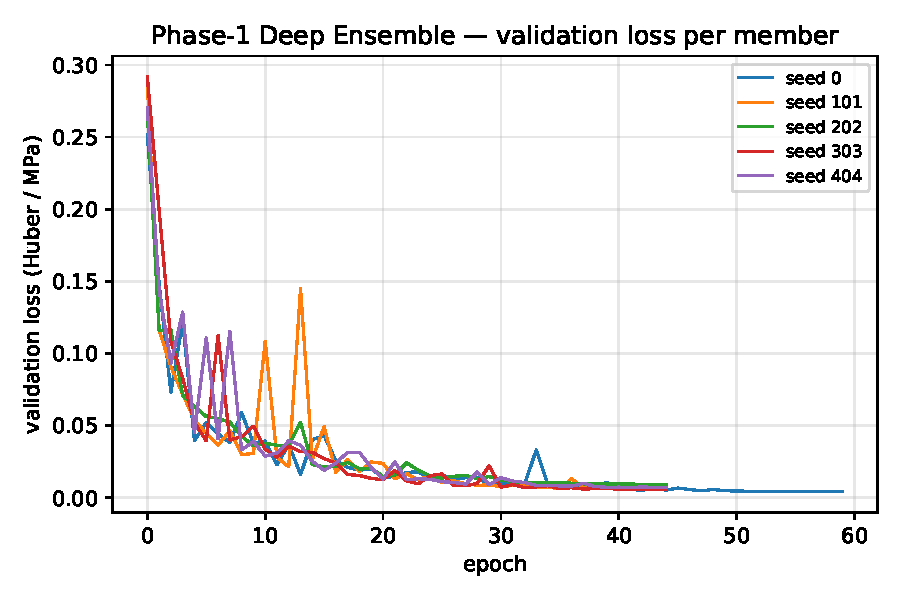
\includegraphics[width=0.7\linewidth]{figures/fig_phase1_training_curves.pdf}
  \caption{Validation loss per epoch for the five Deep-Ensemble members
    (seeds $0, 101, 202, 303, 404$). Huber loss on the un-normalized
    stress target in MPa; cosine schedule with early-stopping patience 12.}
  \label{fig:phase1-curves}
\end{figure}

\section{Full CQR coverage sweep and conditional coverage}
\label{app:cqr}

Table~\ref{tab:coverage-full} extends the three-level coverage summary
of Table~\ref{tab:coverage} to the full four nominal levels swept
($\alpha\in\{0.20, 0.15, 0.10, 0.05\}$). Table~\ref{tab:phase2-conditional}
slices empirical coverage at nominal $90\%$ by quartile of each design
parameter, and Figures~\ref{fig:phase2-interval-width}--\ref{fig:phase2-comparison}
visualize per-sample CQR interval widths, example miscoverage masks,
and the width--vs.--error correspondence that motivates the deferral
rule in Section~\ref{ssec:deferral}.

\begin{table}[h]
  \centering
  \caption{Full four-level CQR coverage sweep (extends
    Table~\ref{tab:coverage}).}
  \label{tab:coverage-full}
  \begin{tabular}{cccccc}
    \toprule
    Nominal [\%] &
    \multicolumn{2}{c}{Uncalibrated (Gaussian)} &
    \multicolumn{2}{c}{CQR-calibrated} &
    $\hat{Q}$ [MPa] \\
    \cmidrule(lr){2-3}\cmidrule(lr){4-5}
    & Coverage & Width [MPa] & Coverage & Width [MPa] & \\
    \midrule
    80 & 86.41 & 0.25 & 82.72 & 0.24 & $-0.005$ \\
    85 & 89.44 & 0.28 & 87.03 & 0.27 & $-0.004$ \\
    90 & 92.32 & 0.32 & 91.28 & 0.31 & $-0.003$ \\
    95 & 95.19 & 0.38 & 95.53 & 0.38 & $\phantom{-}0.001$ \\
    \bottomrule
  \end{tabular}
\end{table}

\begin{table}[h]
  \centering
  \caption{Conditional coverage at nominal $90\%$, sliced by quartile of
    each design parameter. Coverage stays within $\pm 3$~pp of nominal
    across all 12 quartiles.}
  \label{tab:phase2-conditional}
  \begin{tabular}{llccc}
    \toprule
    Slice & Range & $n$ samples & Coverage [\%] & Mean width [MPa] \\
    \midrule
    $R$ Q1 & $[6.51, 7.43]$  & 125 & 91.89 & 0.26 \\
    $R$ Q2 & $[7.43, 8.42]$  & 125 & 92.16 & 0.33 \\
    $R$ Q3 & $[8.42, 9.26]$  & 125 & 91.78 & 0.31 \\
    $R$ Q4 & $[9.26, 10.00]$ & 125 & 89.33 & 0.34 \\
    $p$ Q1 & $[57.02, 61.83]$ & 125 & 91.44 & 0.20 \\
    $p$ Q2 & $[61.83, 66.19]$ & 125 & 91.91 & 0.29 \\
    $p$ Q3 & $[66.19, 69.08]$ & 125 & 91.01 & 0.33 \\
    $p$ Q4 & $[69.08, 72.00]$ & 125 & 90.76 & 0.43 \\
    $W$ Q1 & $[19.01, 20.92]$ & 125 & 90.80 & 0.20 \\
    $W$ Q2 & $[20.92, 22.03]$ & 125 & 92.67 & 0.29 \\
    $W$ Q3 & $[22.03, 23.00]$ & 125 & 91.71 & 0.34 \\
    $W$ Q4 & $[23.00, 24.00]$ & 125 & 89.95 & 0.41 \\
    \bottomrule
  \end{tabular}
\end{table}

\begin{figure}[h]
  \centering
  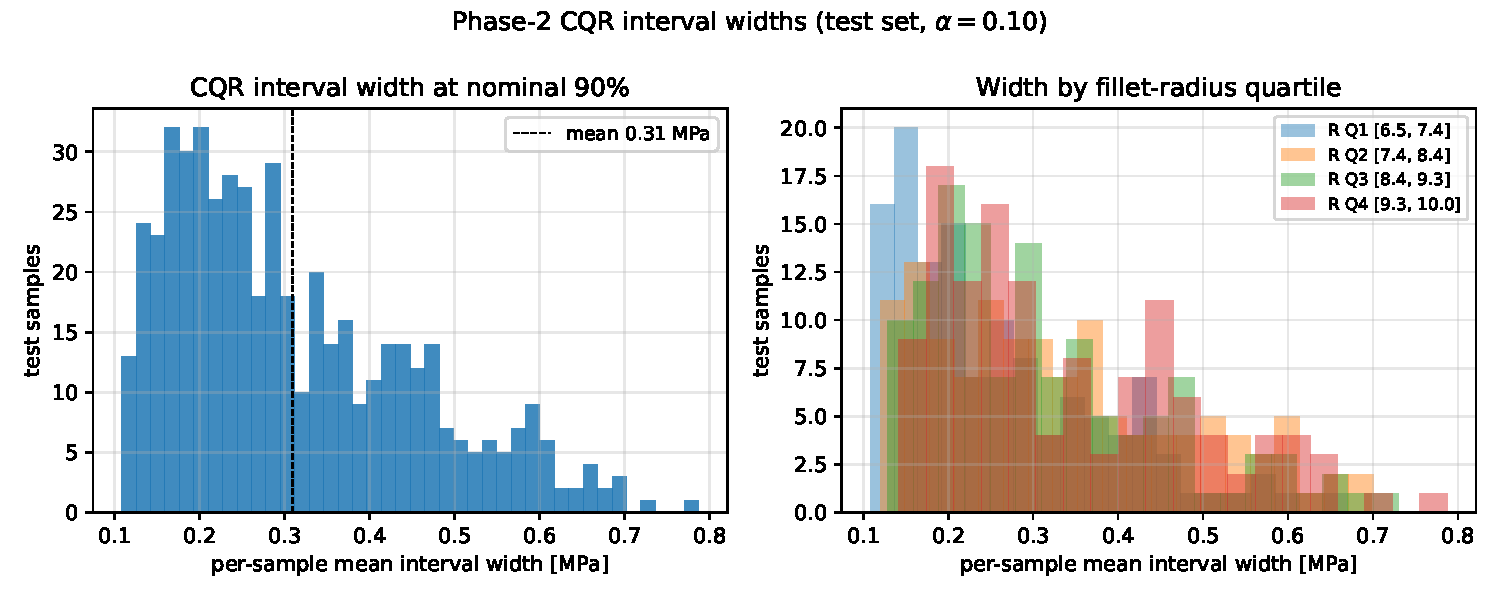
\includegraphics[width=\linewidth]{figures/fig_phase2_interval_width.pdf}
  \caption{Distribution of per-sample mean CQR interval widths on the
    test set at nominal $90\%$. \emph{Left:} pooled over all 500 test
    samples. \emph{Right:} stratified by fillet-radius quartile.}
  \label{fig:phase2-interval-width}
\end{figure}

\begin{figure}[h]
  \centering
  \makebox[\linewidth][c]{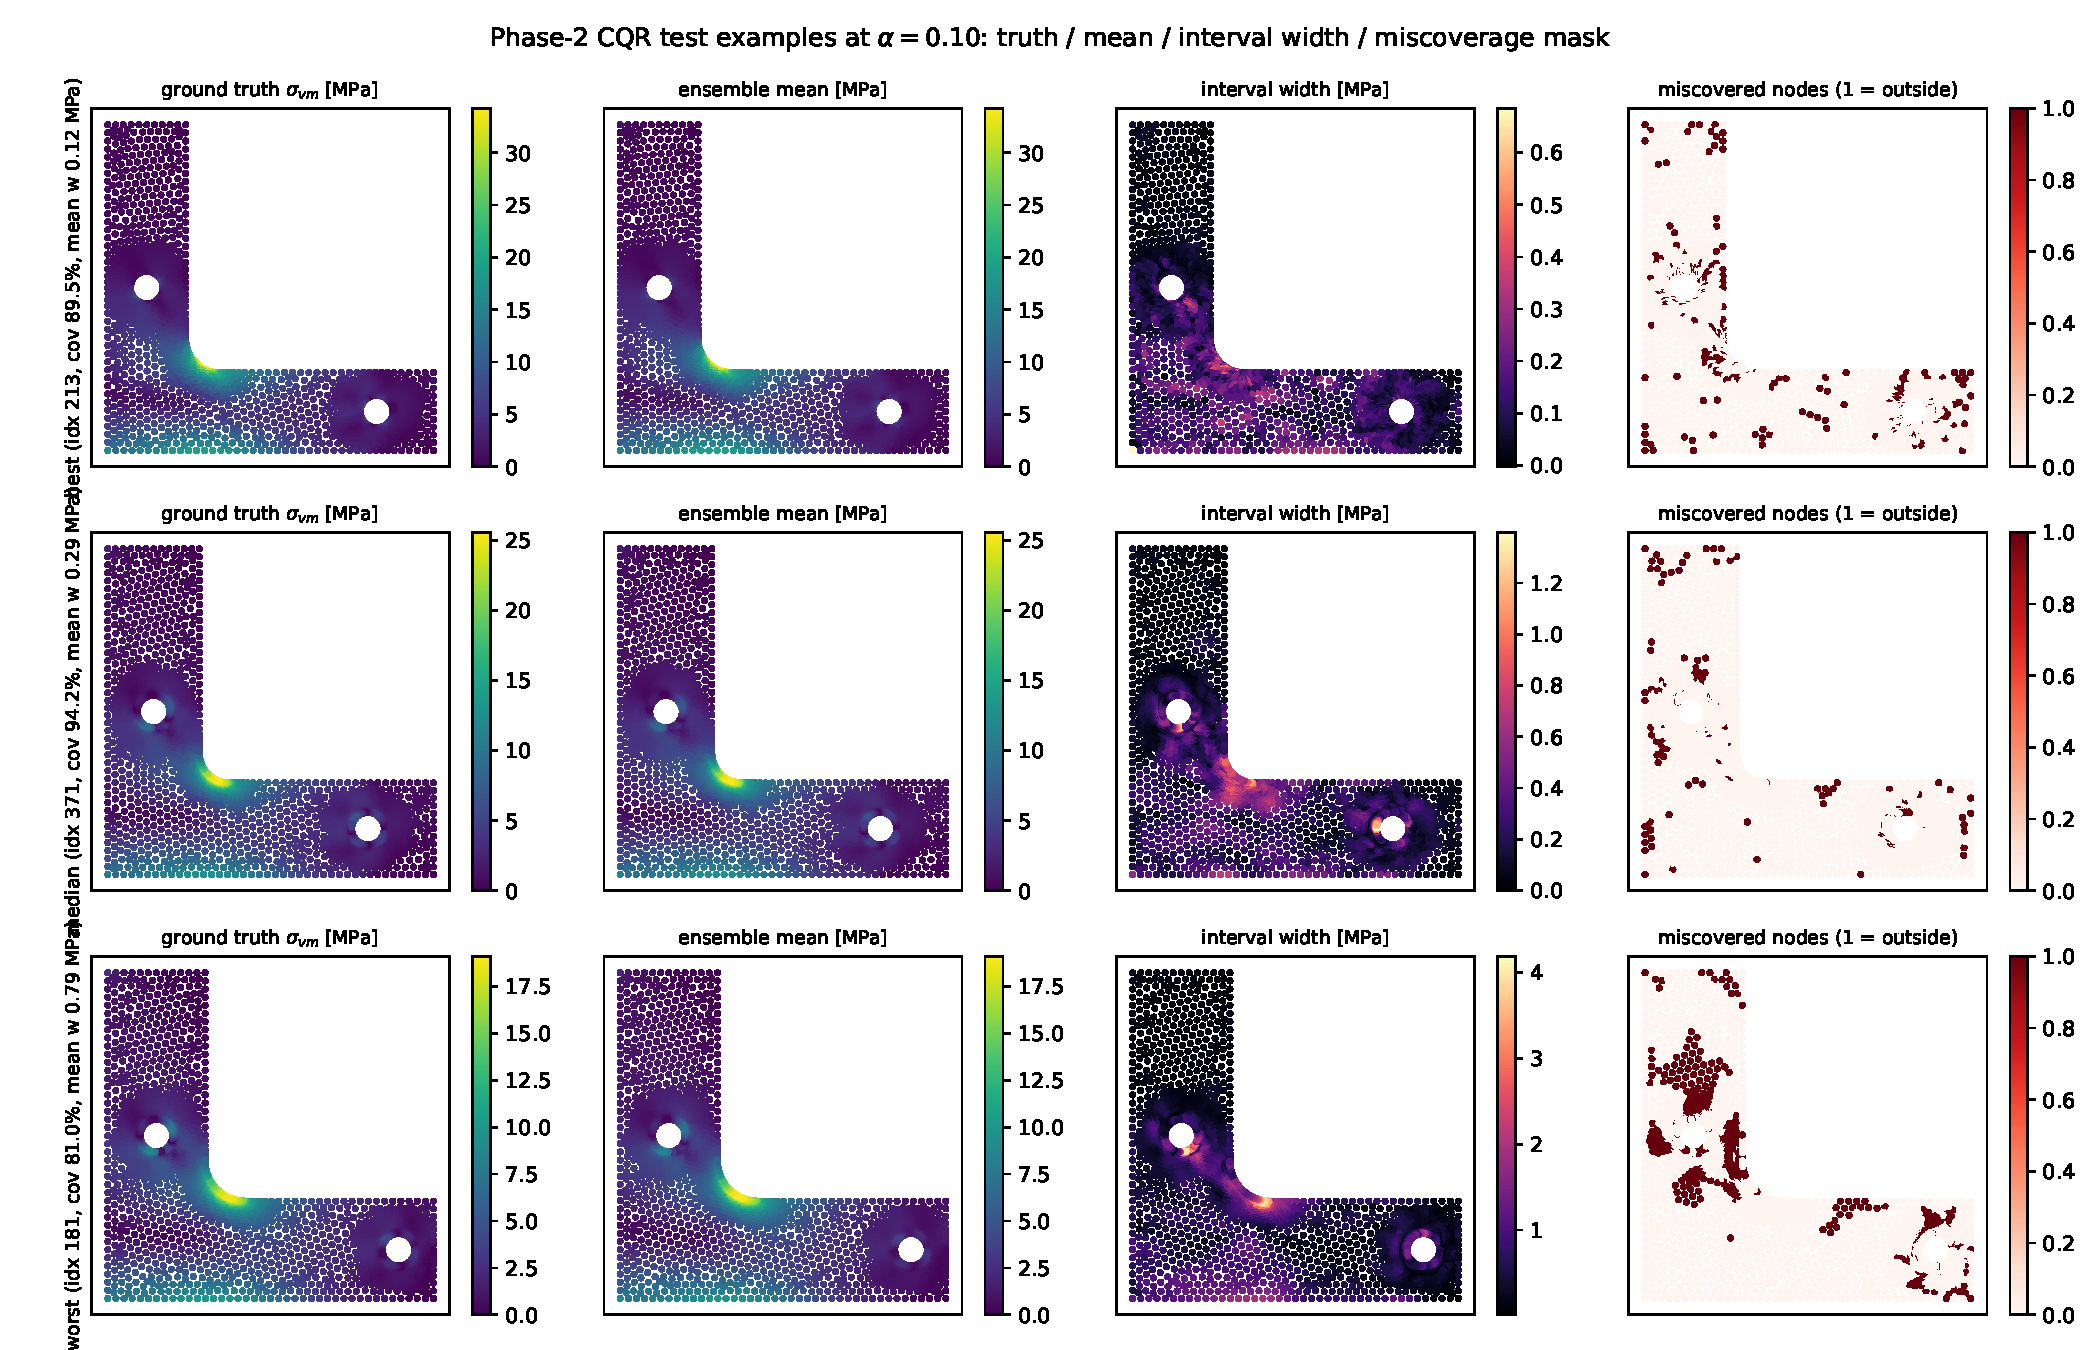
\includegraphics[width=1.15\linewidth]{figures/fig_phase2_intervals_example.pdf}}
  \caption{CQR test-set examples at $\alpha=0.10$ (best, median, worst
    per-sample error). Columns: ground-truth stress; ensemble-mean
    prediction; per-node CQR interval width; miscoverage mask (red = true
    stress outside interval).}
  \label{fig:phase2-intervals-example}
\end{figure}

\begin{figure}[h]
  \centering
  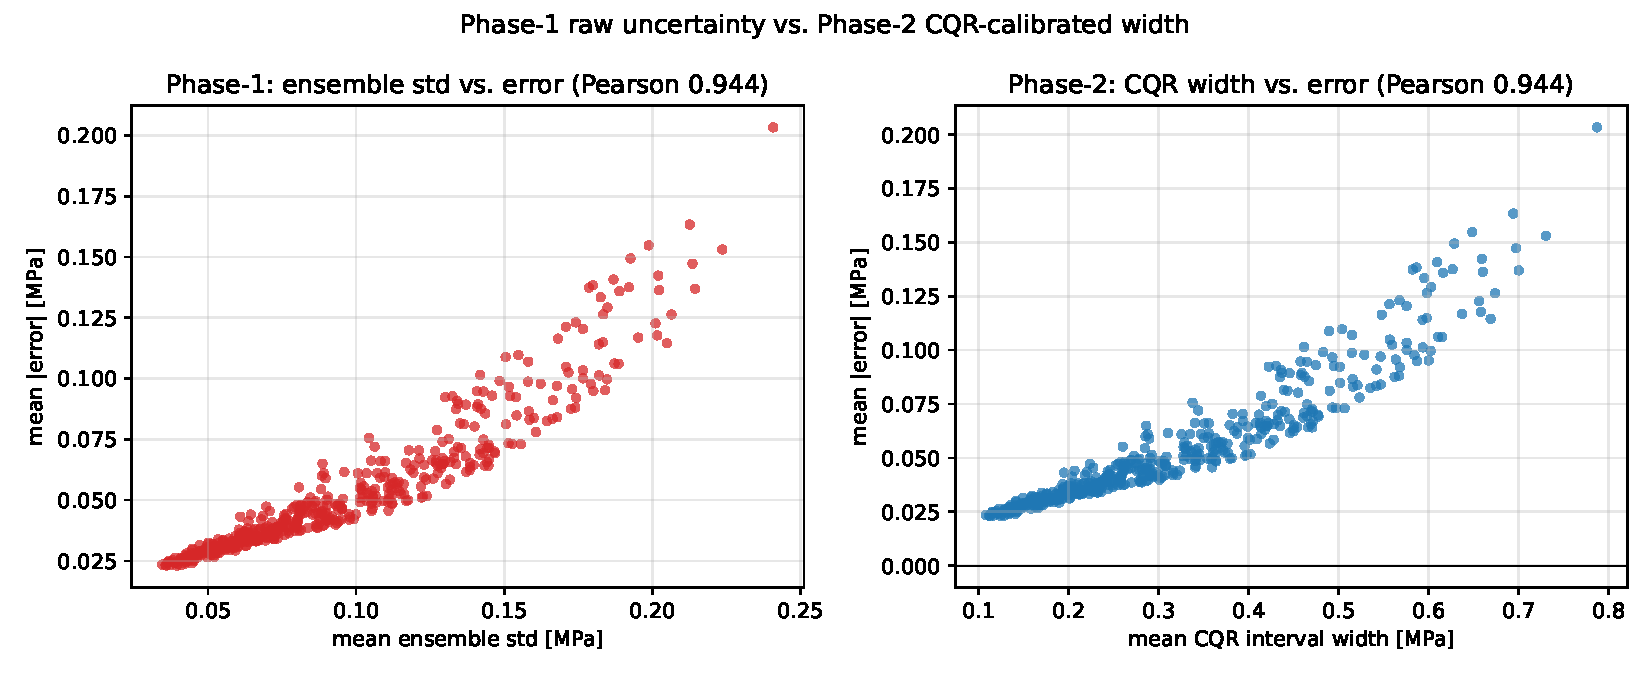
\includegraphics[width=\linewidth]{figures/fig_phase2_comparison.pdf}
  \caption{Phase-1 raw ensemble-std uncertainty (left) vs.\ Phase-2
    CQR-calibrated interval width (right), plotted against per-sample
    mean absolute error on the test set.}
  \label{fig:phase2-comparison}
\end{figure}

\section{OOD per-condition breakdown}
\label{app:ood}

Table~\ref{tab:phase3-conditional} reports accuracy, CQR coverage,
mean interval width, ensemble std, and deferral-rule detection rate
for each of the seven pre-registered OOD conditions (six single-parameter
directions plus the corner condition where two or more parameters are
simultaneously outside the training box).
Figures~\ref{fig:phase3-id-vs-ood-accuracy}--\ref{fig:phase3-ood-examples}
visualize the ID-vs-OOD comparison, the per-direction breakdown, and
three representative OOD predictions (best, median, worst by mean
absolute error).

\begin{table}[h]
  \centering
  \caption{Per-condition OOD breakdown at nominal $90\%$ coverage.}
  \label{tab:phase3-conditional}
  \resizebox{\textwidth}{!}{%
  \begin{tabular}{lcccccc}
    \toprule
    Condition & $n$ & Per-node MAPE [\%] & Coverage [\%]
      & Width [MPa] & Ens.\ std [MPa] & Detection [\%] \\
    \midrule
    $R$-low  & 25 & 1.08 & 88.10 & 0.255 & 0.079 & 0.0 \\
    $R$-high & 25 & 1.29 & 89.21 & 0.249 & 0.077 & 0.0 \\
    $p$-low  & 25 & 2.72 & 84.27 & 0.663 & 0.203 & 44.0 \\
    $p$-high & 25 & 2.72 & 81.36 & 0.242 & 0.075 & 4.0 \\
    $W$-low  & 25 & 2.63 & 78.17 & 0.658 & 0.201 & 44.0 \\
    $W$-high & 25 & 2.35 & 88.77 & 0.369 & 0.114 & 16.0 \\
    Corner ($\geq 2$ OOD) & 100 & 4.56 & 81.46 & 1.085 & 0.332 & 58.0 \\
    \bottomrule
  \end{tabular}%
  }
\end{table}

\begin{figure}[h]
  \centering
  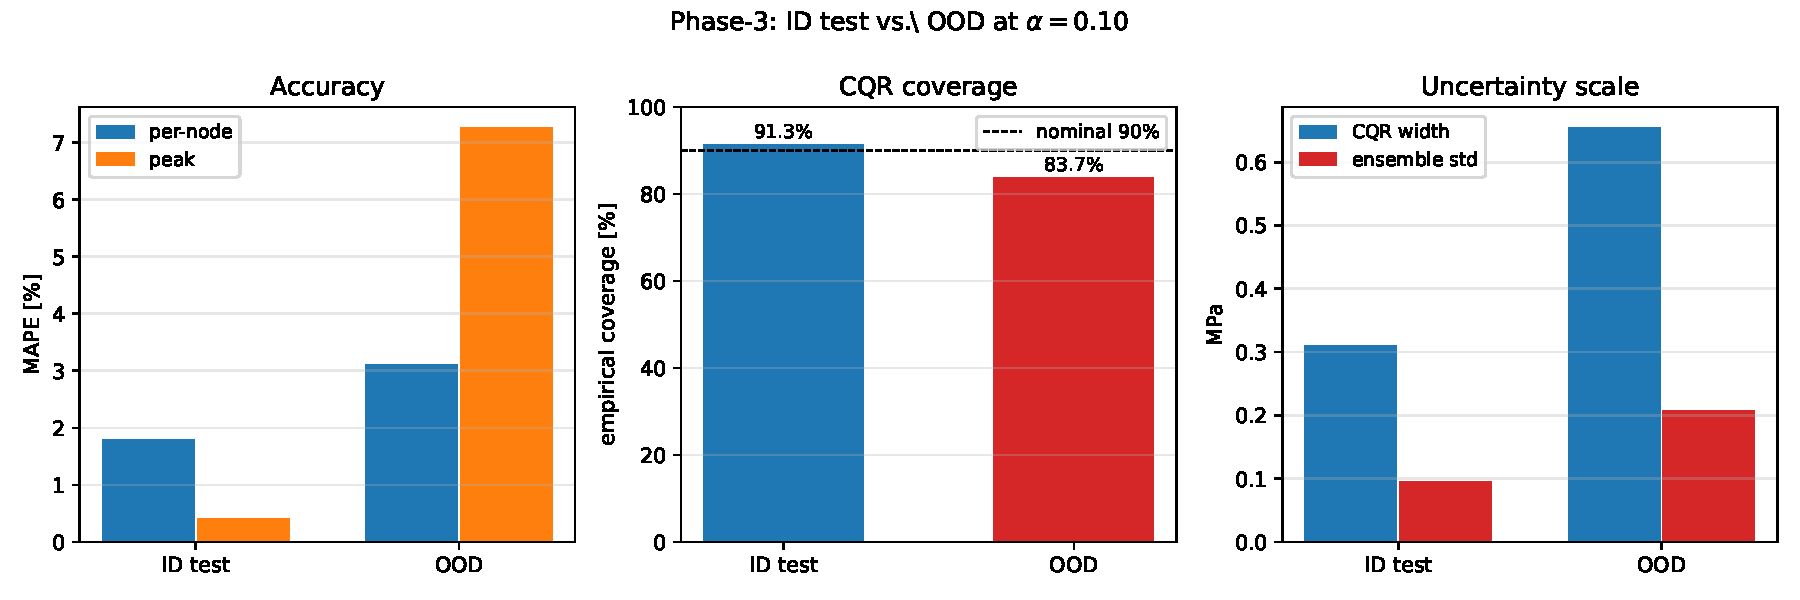
\includegraphics[width=\linewidth]{figures/fig_phase3_id_vs_ood_accuracy.pdf}
  \caption{ID test vs.\ OOD at nominal $90\%$ coverage: per-node and
    peak-stress MAPE, empirical coverage, and interval width / ensemble std.}
  \label{fig:phase3-id-vs-ood-accuracy}
\end{figure}

\begin{figure}[h]
  \centering
  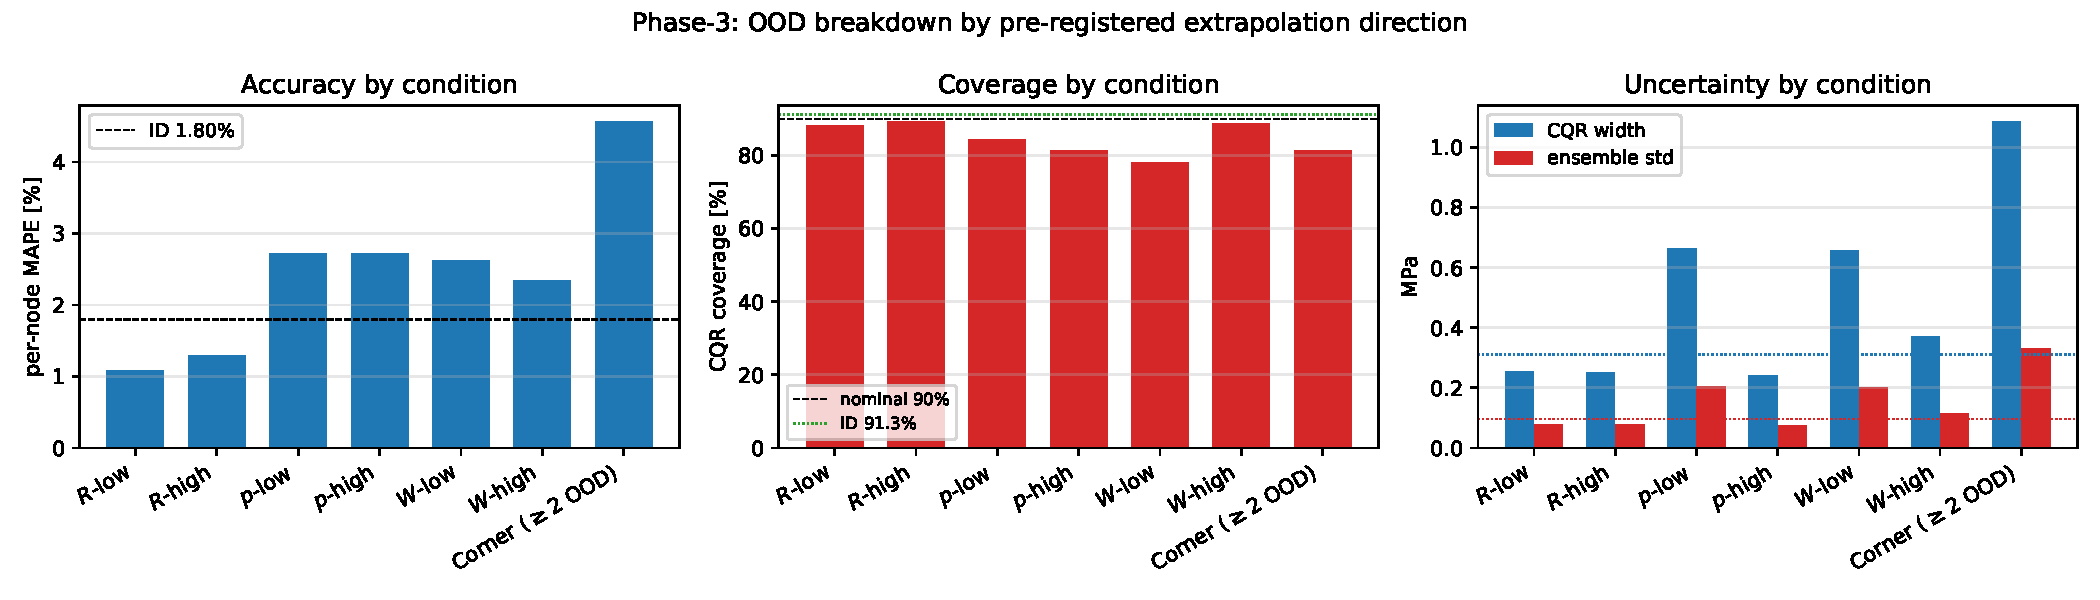
\includegraphics[width=\linewidth]{figures/fig_phase3_ood_breakdown.pdf}
  \caption{OOD metrics broken down by pre-registered extrapolation
    direction. $R$-direction extrapolation is handled well; $p$-low,
    $W$-low, and corner OOD drive the aggregate degradation.}
  \label{fig:phase3-ood-breakdown}
\end{figure}

\begin{figure}[h]
  \centering
  \makebox[\linewidth][c]{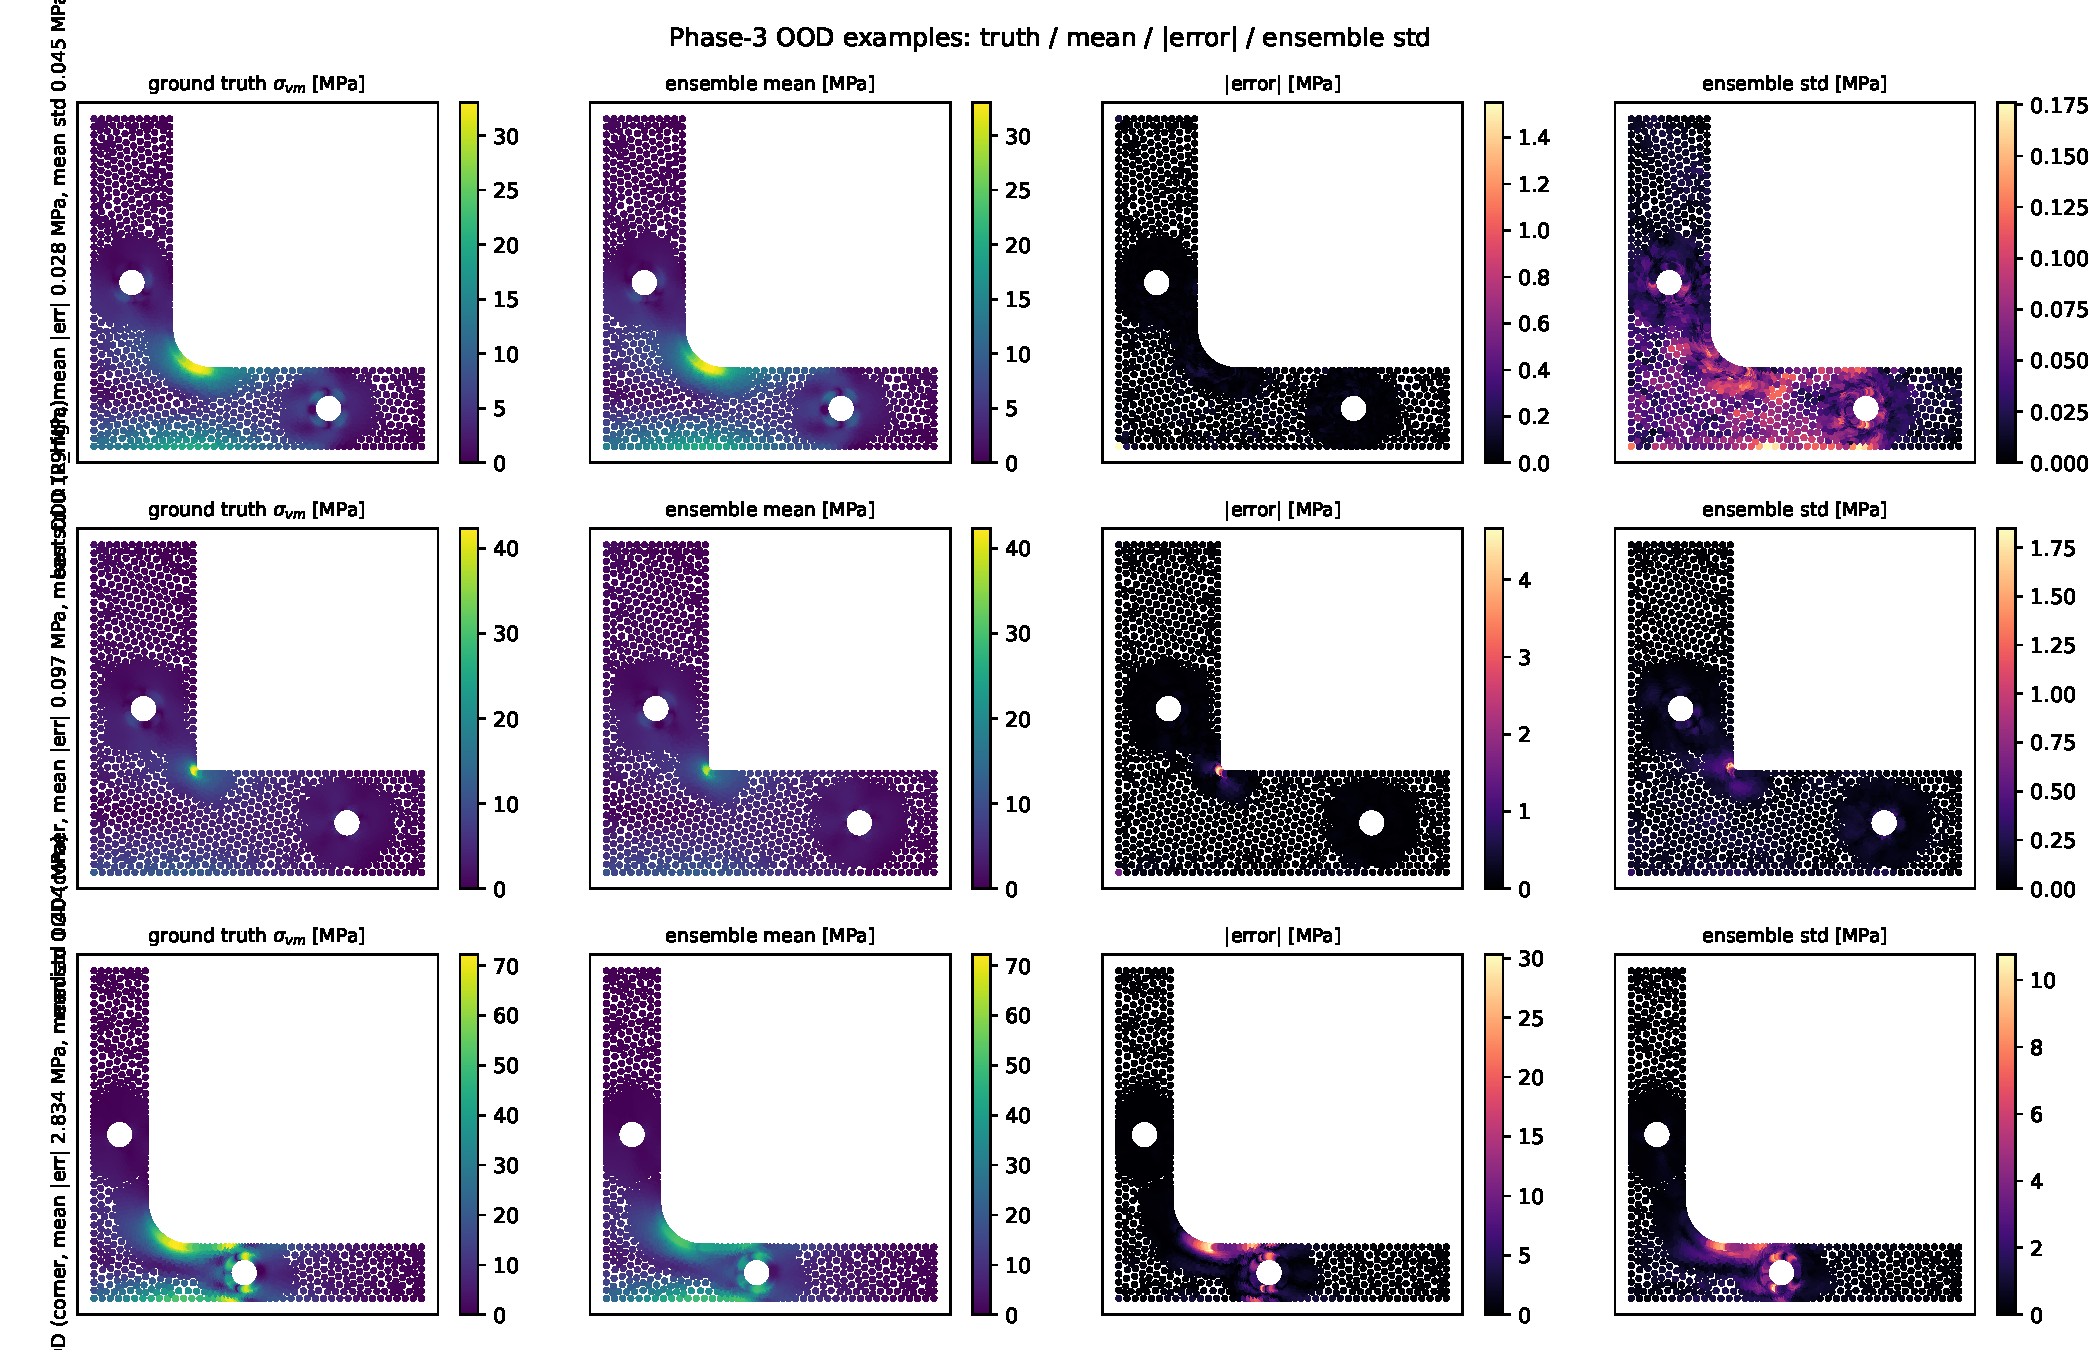
\includegraphics[width=1.15\linewidth]{figures/fig_phase3_ood_examples.pdf}}
  \caption{OOD example stress fields (best, median, worst by mean
    absolute error). Error and std maps are visibly broader than ID and
    migrate off the fillet onto the full bulk field in the worst
    sample.}
  \label{fig:phase3-ood-examples}
\end{figure}

\section{Deferral rule operating characteristic}
\label{app:deferral}

Table~\ref{tab:phase3-deferral} reports the ID false-alarm and OOD
detection rates at four candidate thresholds (ID-std quantiles 80\%,
90\%, 95\%, 99\%); the deployment operating point is the $95^{\text{th}}$
percentile, which by construction yields $5\%$ ID false-alarm.
Figure~\ref{fig:phase3-deferral-roc} shows the corresponding ROC of
per-sample mean ensemble std as an OOD detector, together with the
density of ensemble-std values for ID vs.\ OOD samples.

\begin{table}[h]
  \centering
  \caption{Deferral operating points at four candidate ID-std quantile
    thresholds. The ID false-alarm row is $1-q$ by construction.}
  \label{tab:phase3-deferral}
  \begin{tabular}{lcc}
    \toprule
    Threshold (ID quantile) & ID false-alarm [\%] & OOD detection [\%] \\
    \midrule
    80\% ($T = 0.134$~MPa) & 20.0 & 45.2 \\
    90\% ($T = 0.160$~MPa) & 10.0 & 37.2 \\
    95\% ($T = 0.182$~MPa) & 5.0  & 34.0 \\
    99\% ($T = 0.207$~MPa) & 1.0  & 27.6 \\
    \bottomrule
  \end{tabular}
\end{table}

\begin{figure}[h]
  \centering
  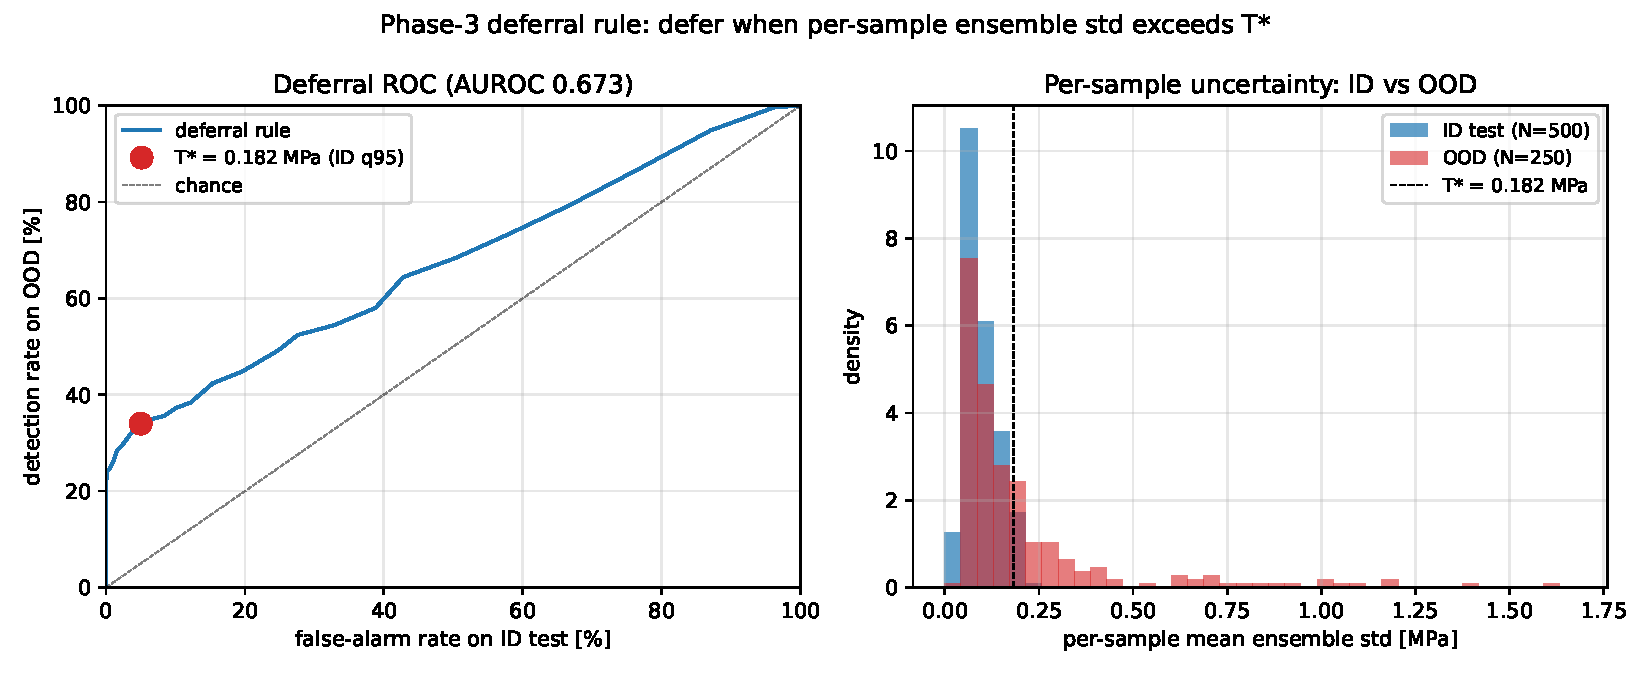
\includegraphics[width=\linewidth]{figures/fig_phase3_deferral_roc.pdf}
  \caption{Defer-to-FEA decision rule. \emph{Left:} ROC of the
    per-sample mean ensemble std as an OOD detector; the marker shows
    the deployment operating point at $T^\star =$ ID-std
    $95^{\text{th}}$ percentile. \emph{Right:} density of per-sample
    ensemble std for ID vs.\ OOD.}
  \label{fig:phase3-deferral-roc}
\end{figure}

\section{Vanilla split-conformal comparison}
\label{app:vanilla}

As a minimal-baseline reference for CQR we evaluate vanilla
split-conformal prediction: taking $E_i = |\bar{\sigma} - \sigma^\star|$
on the validation set as the nonconformity score, calibrating
$Q_{\text{vanilla}}(\alpha)$ via the standard finite-sample corrected
quantile, and constructing constant-width symmetric intervals
$[\bar{\sigma} - Q_{\text{vanilla}},\ \bar{\sigma} + Q_{\text{vanilla}}]$
on the test set. This interval cannot adapt to local heteroscedasticity
by construction (Table~\ref{tab:vanilla-vs-cqr}).

\begin{table}[h]
  \centering
  \caption{Vanilla split-conformal (constant-width) vs.\ CQR
    (adaptive-width) on the ID test set, cell-wise pooled. $2Q$ and
    width are reported in MPa.}
  \label{tab:vanilla-vs-cqr}
  \resizebox{\textwidth}{!}{%
  \begin{tabular}{cccccc}
    \toprule
    Nominal [\%] &
    \multicolumn{3}{c}{Vanilla split-conformal} &
    \multicolumn{2}{c}{CQR} \\
    \cmidrule(lr){2-4}\cmidrule(lr){5-6}
    & Coverage [\%] & $Q_{\text{vanilla}}$ [MPa] & $2Q$ width [MPa]
    & Coverage [\%] & Mean width [MPa] \\
    \midrule
    80 & 68.66 & 0.056 & 0.111 & 82.72 & 0.236 \\
    90 & 81.07 & 0.084 & 0.167 & 91.28 & 0.311 \\
    95 & 89.02 & 0.118 & 0.236 & 95.53 & 0.379 \\
    \bottomrule
  \end{tabular}%
  }
\end{table}

Vanilla split-conformal produces narrower intervals but under-covers
the nominal level: the $\alpha=0.10$ interval achieves $81.1\%$
empirical coverage instead of $90\%$. The Romano Theorem~1 guarantee
still holds at the point level of exchangeable units, but the cell-wise
pooling used here treats mesh nodes within a graph as exchangeable
when they are in fact correlated within each sample. CQR's adaptive
width --- wider on high-uncertainty regions and samples --- absorbs
this within-sample correlation and recovers nominal coverage. This is
exactly the deployment-relevant property CQR adds beyond the simplest
conformal baseline: adaptive intervals that remain valid when the
exchangeability assumption is only approximately met.

\section{Ensemble-size ablation}
\label{app:ensemble-ablation}

We re-use the frozen 5-member ensemble to evaluate the effect of
ensemble size $M \in \{2, 3, 4, 5\}$ on accuracy and CQR coverage at
$\alpha=0.10$. For each $M$, we take the first $M$ seeds from
$\{0, 101, 202, 303, 404\}$, recompute the ensemble mean and std,
re-run the CQR calibration on the 500-sample validation set, and
evaluate on the test set (Table~\ref{tab:ensemble-ablation}). No
retraining is performed.

\begin{table}[h]
  \centering
  \caption{Ensemble-size ablation on the ID test set at nominal $90\%$
    coverage. $\hat{Q}$ and width are reported in MPa.}
  \label{tab:ensemble-ablation}
  \resizebox{\textwidth}{!}{%
  \begin{tabular}{cccccc}
    \toprule
    $M$ & Per-node MAPE [\%] & Peak-stress MAPE [\%] & CQR coverage [\%]
      & Mean width [MPa] & Mean ens.\ std [MPa] \\
    \midrule
    2 & 1.98 & 0.32 & 86.45 & 0.252 & 0.050 \\
    3 & 2.10 & 0.32 & 88.35 & 0.292 & 0.079 \\
    4 & 1.89 & 0.52 & 90.40 & 0.308 & 0.091 \\
    5 & \textbf{1.81} & 0.42 & \textbf{91.28} & 0.311 & 0.096 \\
    \bottomrule
  \end{tabular}%
  }
\end{table}

Both accuracy (per-node MAPE) and calibration quality (CQR coverage at
$90\%$) improve monotonically from $M=3$ onward. $M=5$ delivers the
best per-node MAPE and the best CQR coverage, confirming the
Lakshminarayanan~\citep{lakshminarayanan2017ensembles} recommendation
of 5-member ensembles as a robust practical choice. The mean ensemble
std grows with $M$ as expected (small-$M$ ensembles under-estimate
variance), which explains the widening CQR interval with $M$; the net
effect is better-calibrated coverage rather than over-wide intervals.

\end{document}
